\documentclass[11pt]{article}
\usepackage[margin=1in]{geometry}
\usepackage[T1]{fontenc}
\usepackage{amsmath,amssymb,amsthm}
\usepackage{graphicx}
\usepackage{booktabs}
\usepackage{algorithm}
\usepackage{algpseudocode}
\usepackage{xspace}
\usepackage[hidelinks]{hyperref}

\newtheorem{theorem}{Theorem}
\newtheorem{proposition}{Proposition}
\newtheorem{observation}{Observation}
\newcommand{\cs}{\textsc{CoStrata}\xspace}
\newcommand{\omni}{OmniSketch\xspace}
\newcommand{\E}{\mathbb{E}}
\newcommand{\Var}{\mathrm{Var}}
\newcommand{\nstar}{n^{\star}}
% generated by scripts/plots.py -- do not edit
\newcommand{\NumAnchorNeutralMawiHi}{1.12}
\newcommand{\NumAnchorNeutralMawiLo}{0.90}
\newcommand{\NumAnchorNeutralZipfFifteenHi}{2.85}
\newcommand{\NumAnchorNeutralZipfFifteenLo}{0.74}
\newcommand{\NumAshLeanVsResGm}{0.88}
\newcommand{\NumAshLeanVsResHi}{2.33}
\newcommand{\NumAshLeanVsResLo}{0.18}
\newcommand{\NumAshVsResGm}{1.28}
\newcommand{\NumAshVsResHi}{2.21}
\newcommand{\NumAshVsResLo}{0.31}
\newcommand{\NumBestRowVsResGm}{4.2}
\newcommand{\NumBestRowVsResHi}{29.9}
\newcommand{\NumBestRowVsResLo}{1.2}
\newcommand{\NumBestVariantCells}{45}
\newcommand{\NumBestVariantJavaCount}{0}
\newcommand{\NumBiasCalTotalHoldMawi}{+0.01}
\newcommand{\NumBiasCalTotalHoldTaxi}{-0.00}
\newcommand{\NumBiasCalTotalHoldZipf}{+0.01}
\newcommand{\NumBiasCalTotalMawi}{-0.01}
\newcommand{\NumBiasCalTotalSeHoldMawi}{0.00}
\newcommand{\NumBiasCalTotalSeHoldTaxi}{0.01}
\newcommand{\NumBiasCalTotalSeHoldZipf}{0.01}
\newcommand{\NumBiasCalTotalSeMawi}{0.01}
\newcommand{\NumBiasCalTotalSeTaxi}{0.00}
\newcommand{\NumBiasCalTotalSeZipf}{0.02}
\newcommand{\NumBiasCalTotalTaxi}{-0.00}
\newcommand{\NumBiasCalTotalZipf}{+0.01}
\newcommand{\NumBiasHtTotalHoldMawi}{+0.03}
\newcommand{\NumBiasHtTotalHoldTaxi}{+0.04}
\newcommand{\NumBiasHtTotalHoldZipf}{+0.04}
\newcommand{\NumBiasHtTotalMawi}{+0.03}
\newcommand{\NumBiasHtTotalSeHoldMawi}{0.02}
\newcommand{\NumBiasHtTotalSeHoldTaxi}{0.04}
\newcommand{\NumBiasHtTotalSeHoldZipf}{0.05}
\newcommand{\NumBiasHtTotalSeMawi}{0.05}
\newcommand{\NumBiasHtTotalSeTaxi}{0.04}
\newcommand{\NumBiasHtTotalSeZipf}{0.06}
\newcommand{\NumBiasHtTotalTaxi}{+0.03}
\newcommand{\NumBiasHtTotalZipf}{-0.07}
\newcommand{\NumBiasHtZHoldMawi}{96}
\newcommand{\NumBiasHtZHoldTaxi}{92}
\newcommand{\NumBiasHtZHoldZipf}{95}
\newcommand{\NumBiasHtZMawi}{95}
\newcommand{\NumBiasHtZTaxi}{94}
\newcommand{\NumBiasHtZZipf}{94}
\newcommand{\NumBiasQueriesHoldMawi}{1352}
\newcommand{\NumBiasQueriesHoldTaxi}{1072}
\newcommand{\NumBiasQueriesHoldZipf}{697}
\newcommand{\NumBiasQueriesMawi}{1352}
\newcommand{\NumBiasQueriesTaxi}{1072}
\newcommand{\NumBiasQueriesZipf}{697}
\newcommand{\NumBiasSeedsHoldMawi}{300}
\newcommand{\NumBiasSeedsHoldTaxi}{600}
\newcommand{\NumBiasSeedsHoldZipf}{300}
\newcommand{\NumBiasSeedsMawi}{300}
\newcommand{\NumBiasSeedsTaxi}{600}
\newcommand{\NumBiasSeedsZipf}{300}
\newcommand{\NumCalOneKoneGm}{19}
\newcommand{\NumCalOneKoneHi}{3385}
\newcommand{\NumCalOneKoneLo}{1}
\newcommand{\NumCalOneKtwoGm}{1.31}
\newcommand{\NumCalOneKtwoHi}{3.93}
\newcommand{\NumCalOneKtwoLo}{0.82}
\newcommand{\NumCalOneVsResAllGm}{2.15}
\newcommand{\NumCalOneVsResAllHi}{4.70}
\newcommand{\NumCalOneVsResAllLo}{0.90}
\newcommand{\NumCalOneVsResGm}{1.16}
\newcommand{\NumCalOneVsResHi}{2.33}
\newcommand{\NumCalOneVsResLo}{0.78}
\newcommand{\NumCalOneVsResMawiGm}{2.01}
\newcommand{\NumCalOneVsResMawiHi}{2.33}
\newcommand{\NumCalOneVsResMawiLo}{1.46}
\newcommand{\NumCalOneVsResTaxiGm}{1.23}
\newcommand{\NumCalOneVsResTaxiHi}{1.35}
\newcommand{\NumCalOneVsResTaxiLo}{1.16}
\newcommand{\NumCalOneVsResZipfFifteenGm}{0.97}
\newcommand{\NumCalOneVsResZipfFifteenHi}{1.04}
\newcommand{\NumCalOneVsResZipfFifteenLo}{0.89}
\newcommand{\NumCalOneVsResZipfTenGm}{0.87}
\newcommand{\NumCalOneVsResZipfTenHi}{0.93}
\newcommand{\NumCalOneVsResZipfTenLo}{0.83}
\newcommand{\NumCalOneVsResZipfThirteenGm}{0.93}
\newcommand{\NumCalOneVsResZipfThirteenHi}{0.97}
\newcommand{\NumCalOneVsResZipfThirteenLo}{0.88}
\newcommand{\NumCalThreeKfourGm}{1.40}
\newcommand{\NumCalThreeKfourHi}{8.38}
\newcommand{\NumCalThreeKfourLo}{0.58}
\newcommand{\NumCalThreeKthreeGm}{3.8}
\newcommand{\NumCalThreeKthreeHi}{21.2}
\newcommand{\NumCalThreeKthreeLo}{0.7}
\newcommand{\NumCalThreeVsCalTwoGm}{1.33}
\newcommand{\NumCalThreeVsCalTwoHi}{2.60}
\newcommand{\NumCalThreeVsCalTwoLo}{0.83}
\newcommand{\NumCalThreeVsResGm}{3.6}
\newcommand{\NumCalThreeVsResHi}{12.9}
\newcommand{\NumCalThreeVsResLo}{1.1}
\newcommand{\NumCalTwoKfourGm}{1.27}
\newcommand{\NumCalTwoKfourHi}{6.72}
\newcommand{\NumCalTwoKfourLo}{0.58}
\newcommand{\NumCalTwoKthreeGm}{1.7}
\newcommand{\NumCalTwoKthreeHi}{9.6}
\newcommand{\NumCalTwoKthreeLo}{0.7}
\newcommand{\NumCalTwoKtwoGm}{11}
\newcommand{\NumCalTwoKtwoHi}{144}
\newcommand{\NumCalTwoKtwoLo}{1}
\newcommand{\NumCalTwoVsResGm}{2.7}
\newcommand{\NumCalTwoVsResHi}{11.4}
\newcommand{\NumCalTwoVsResLo}{1.2}
\newcommand{\NumCalTwoVsResMawiGm}{5.2}
\newcommand{\NumCalTwoVsResMawiHi}{11.4}
\newcommand{\NumCalTwoVsResMawiLo}{2.1}
\newcommand{\NumCalTwoVsResTaxiGm}{2.9}
\newcommand{\NumCalTwoVsResTaxiHi}{3.4}
\newcommand{\NumCalTwoVsResTaxiLo}{2.2}
\newcommand{\NumCalTwoVsResUnifGm}{0.94}
\newcommand{\NumCalTwoVsResUnifHi}{1.14}
\newcommand{\NumCalTwoVsResUnifLo}{0.70}
\newcommand{\NumCalTwoVsResZipfFifteenGm}{2.0}
\newcommand{\NumCalTwoVsResZipfFifteenHi}{2.2}
\newcommand{\NumCalTwoVsResZipfFifteenLo}{1.8}
\newcommand{\NumCalTwoVsResZipfTenGm}{1.6}
\newcommand{\NumCalTwoVsResZipfTenHi}{1.9}
\newcommand{\NumCalTwoVsResZipfTenLo}{1.2}
\newcommand{\NumCalTwoVsResZipfThirteenGm}{2.3}
\newcommand{\NumCalTwoVsResZipfThirteenHi}{2.7}
\newcommand{\NumCalTwoVsResZipfThirteenLo}{1.9}
\newcommand{\NumCapKtwoCalOne}{5.9\cdot10^{-4}}
\newcommand{\NumCapKtwoExact}{2.5\cdot10^{-5}}
\newcommand{\NumCapKtwoSampled}{6.4\cdot10^{-4}}
\newcommand{\NumCensusJavaVsResFour}{10.1}
\newcommand{\NumCensusJavaVsResSixtyEight}{190}
\newcommand{\NumCensusOmniAnyVsResFour}{2.7}
\newcommand{\NumCensusOmniAnyVsResSixtyEight}{2.5}
\newcommand{\NumCensusPairWidth}{256}
\newcommand{\NumCensusResVsCalOneFour}{1.2}
\newcommand{\NumCensusResVsCalOneSixtyEight}{1.7}
\newcommand{\NumCensusResVsCalTwoFour}{3.8}
\newcommand{\NumCensusResVsCalTwoSixtyEight}{4.6}
\newcommand{\NumCensusResVsCsFour}{4.0}
\newcommand{\NumCensusResVsCsSixtyEight}{4.4}
\newcommand{\NumCmVsCalTwoGm}{58.6}
\newcommand{\NumCmVsCalTwoHi}{577}
\newcommand{\NumCmVsCalTwoLo}{5.8}
\newcommand{\NumCsThroughput}{??}
\newcommand{\NumCsVsCalTwoGm}{1.10}
\newcommand{\NumCsVsCalTwoHi}{1.29}
\newcommand{\NumCsVsCalTwoLo}{1.00}
\newcommand{\NumCsVsCalTwoMawiGm}{1.04}
\newcommand{\NumCsVsCalTwoMawiHi}{1.06}
\newcommand{\NumCsVsCalTwoMawiLo}{1.02}
\newcommand{\NumCsVsCalTwoTaxiGm}{1.10}
\newcommand{\NumCsVsCalTwoTaxiHi}{1.18}
\newcommand{\NumCsVsCalTwoTaxiLo}{1.04}
\newcommand{\NumCsVsCalTwoZipfFifteenGm}{1.20}
\newcommand{\NumCsVsCalTwoZipfFifteenHi}{1.29}
\newcommand{\NumCsVsCalTwoZipfFifteenLo}{1.09}
\newcommand{\NumCsVsCalTwoZipfTenGm}{1.04}
\newcommand{\NumCsVsCalTwoZipfTenHi}{1.07}
\newcommand{\NumCsVsCalTwoZipfTenLo}{1.01}
\newcommand{\NumCsVsCalTwoZipfThirteenGm}{1.18}
\newcommand{\NumCsVsCalTwoZipfThirteenHi}{1.23}
\newcommand{\NumCsVsCalTwoZipfThirteenLo}{1.11}
\newcommand{\NumCsVsResGm}{2.4}
\newcommand{\NumCsVsResHi}{11.1}
\newcommand{\NumCsVsResLo}{1.2}
\newcommand{\NumCshVsCalTwoGm}{1.01}
\newcommand{\NumCshVsCalTwoHi}{1.31}
\newcommand{\NumCshVsCalTwoLo}{0.46}
\newcommand{\NumCshVsCsMawiGm}{1.43}
\newcommand{\NumCshVsCsMawiHi}{1.66}
\newcommand{\NumCshVsCsMawiLo}{1.24}
\newcommand{\NumCshVsCsTaxiGm}{0.92}
\newcommand{\NumCshVsCsTaxiHi}{0.95}
\newcommand{\NumCshVsCsTaxiLo}{0.88}
\newcommand{\NumCshVsCsZipfFifteenGm}{1.43}
\newcommand{\NumCshVsCsZipfFifteenHi}{2.38}
\newcommand{\NumCshVsCsZipfFifteenLo}{1.09}
\newcommand{\NumCshVsCsZipfTenGm}{0.91}
\newcommand{\NumCshVsCsZipfTenHi}{0.98}
\newcommand{\NumCshVsCsZipfTenLo}{0.85}
\newcommand{\NumCshVsCsZipfThirteenGm}{0.98}
\newcommand{\NumCshVsCsZipfThirteenHi}{1.09}
\newcommand{\NumCshVsCsZipfThirteenLo}{0.88}
\newcommand{\NumCshVsResMawiGm}{7.1}
\newcommand{\NumCshVsResMawiHi}{18.4}
\newcommand{\NumCshVsResMawiLo}{2.5}
\newcommand{\NumCshVsResTaxiGm}{2.4}
\newcommand{\NumCshVsResTaxiHi}{3.1}
\newcommand{\NumCshVsResTaxiLo}{1.7}
\newcommand{\NumCshVsResZipfFifteenGm}{2.4}
\newcommand{\NumCshVsResZipfFifteenHi}{4.0}
\newcommand{\NumCshVsResZipfFifteenLo}{1.7}
\newcommand{\NumCshVsResZipfTenGm}{1.4}
\newcommand{\NumCshVsResZipfTenHi}{1.6}
\newcommand{\NumCshVsResZipfTenLo}{1.0}
\newcommand{\NumCshVsResZipfThirteenGm}{1.9}
\newcommand{\NumCshVsResZipfThirteenHi}{2.4}
\newcommand{\NumCshVsResZipfThirteenLo}{1.6}
\newcommand{\NumCshVsUssCalTwoMawiGm}{1.37}
\newcommand{\NumCshVsUssCalTwoMawiHi}{1.62}
\newcommand{\NumCshVsUssCalTwoMawiLo}{1.27}
\newcommand{\NumCshVsUssCalTwoTaxiGm}{1.26}
\newcommand{\NumCshVsUssCalTwoTaxiHi}{1.35}
\newcommand{\NumCshVsUssCalTwoTaxiLo}{1.21}
\newcommand{\NumCshVsUssCalTwoZipfFifteenGm}{1.85}
\newcommand{\NumCshVsUssCalTwoZipfFifteenHi}{2.05}
\newcommand{\NumCshVsUssCalTwoZipfFifteenLo}{1.62}
\newcommand{\NumCshVsUssCalTwoZipfTenGm}{1.13}
\newcommand{\NumCshVsUssCalTwoZipfTenHi}{1.18}
\newcommand{\NumCshVsUssCalTwoZipfTenLo}{1.09}
\newcommand{\NumCshVsUssCalTwoZipfThirteenGm}{1.48}
\newcommand{\NumCshVsUssCalTwoZipfThirteenHi}{1.58}
\newcommand{\NumCshVsUssCalTwoZipfThirteenLo}{1.26}
\newcommand{\NumCshWorstFactor}{2.8}
\newcommand{\NumFigSixUnifFifty}{3.8\cdot10^{-7}}
\newcommand{\NumFigSixUnifHundred}{4.4\cdot10^{-7}}
\newcommand{\NumFigSixUnifTen}{3.6\cdot10^{-7}}
\newcommand{\NumFigSixZipfFifteenFifty}{2.4\cdot10^{-4}}
\newcommand{\NumFigSixZipfFifteenHundred}{2.0\cdot10^{-4}}
\newcommand{\NumFigSixZipfFifteenTen}{4.5\cdot10^{-4}}
\newcommand{\NumFigSixZipfTenFifty}{1.2\cdot10^{-5}}
\newcommand{\NumFigSixZipfTenHundred}{9.4\cdot10^{-6}}
\newcommand{\NumFigSixZipfTenTen}{1.4\cdot10^{-5}}
\newcommand{\NumFigSixZipfThirteenFifty}{1.0\cdot10^{-4}}
\newcommand{\NumFigSixZipfThirteenHundred}{8.2\cdot10^{-5}}
\newcommand{\NumFigSixZipfThirteenTen}{1.5\cdot10^{-4}}
\newcommand{\NumHtBiasMax}{1.7}
\newcommand{\NumHtVsCalMawi}{11.4}
\newcommand{\NumHtVsCalTaxi}{7.5}
\newcommand{\NumHtVsCalZipf}{4.7}
\newcommand{\NumHydraVsCalThreeGm}{1.67}
\newcommand{\NumHydraVsCalThreeHi}{3.14}
\newcommand{\NumHydraVsCalThreeLo}{0.57}
\newcommand{\NumHydraVsCalTwoGm}{1.04}
\newcommand{\NumHydraVsCalTwoHi}{3.50}
\newcommand{\NumHydraVsCalTwoLo}{0.23}
\newcommand{\NumJRAshLeanVsResGm}{1.25}
\newcommand{\NumJRAshLeanVsResHi}{1.38}
\newcommand{\NumJRAshLeanVsResLo}{1.18}
\newcommand{\NumJRAshVsResGm}{1.85}
\newcommand{\NumJRAshVsResHi}{2.02}
\newcommand{\NumJRAshVsResLo}{1.73}
\newcommand{\NumJRCalTwoVsResGm}{3.1}
\newcommand{\NumJRCalTwoVsResHi}{3.2}
\newcommand{\NumJRCalTwoVsResLo}{3.0}
\newcommand{\NumJROmniVsAshGm}{3.6}
\newcommand{\NumJROmniVsAshHi}{4.2}
\newcommand{\NumJROmniVsAshLo}{3.1}
\newcommand{\NumJROmniVsResGm}{6.6}
\newcommand{\NumJROmniVsResHi}{8.5}
\newcommand{\NumJROmniVsResLo}{5.7}
\newcommand{\NumJROmniVsResjGm}{4.0}
\newcommand{\NumJROmniVsResjHi}{4.4}
\newcommand{\NumJROmniVsResjLo}{3.8}
\newcommand{\NumJRPvldbVsResGm}{27.1}
\newcommand{\NumJRPvldbVsResHi}{50.0}
\newcommand{\NumJRPvldbVsResLo}{15.7}
\newcommand{\NumJRResjVsResGm}{1.64}
\newcommand{\NumJRResjVsResHi}{1.92}
\newcommand{\NumJRResjVsResLo}{1.44}
\newcommand{\NumJSAshLeanVsResGm}{1.25}
\newcommand{\NumJSAshLeanVsResHi}{1.37}
\newcommand{\NumJSAshLeanVsResLo}{1.16}
\newcommand{\NumJSAshVsResGm}{1.92}
\newcommand{\NumJSAshVsResHi}{2.18}
\newcommand{\NumJSAshVsResLo}{1.76}
\newcommand{\NumJSCalTwoVsResGm}{4.2}
\newcommand{\NumJSCalTwoVsResHi}{4.5}
\newcommand{\NumJSCalTwoVsResLo}{3.9}
\newcommand{\NumJSMreAsh}{1.65}
\newcommand{\NumJSMreCalTwo}{1.34}
\newcommand{\NumJSMreOmni}{1.54}
\newcommand{\NumJSMreRes}{1.41}
\newcommand{\NumJSMreResj}{1.64}
\newcommand{\NumJSOmniVsAshGm}{2.5}
\newcommand{\NumJSOmniVsAshHi}{2.9}
\newcommand{\NumJSOmniVsAshLo}{2.1}
\newcommand{\NumJSOmniVsResGm}{4.8}
\newcommand{\NumJSOmniVsResHi}{6.3}
\newcommand{\NumJSOmniVsResLo}{4.1}
\newcommand{\NumJSOmniVsResjGm}{3.0}
\newcommand{\NumJSOmniVsResjHi}{3.2}
\newcommand{\NumJSOmniVsResjLo}{2.7}
\newcommand{\NumJSPvldbVsResGm}{55.9}
\newcommand{\NumJSPvldbVsResHi}{118}
\newcommand{\NumJSPvldbVsResLo}{28.9}
\newcommand{\NumJSResjVsResGm}{1.60}
\newcommand{\NumJSResjVsResHi}{1.97}
\newcommand{\NumJSResjVsResLo}{1.43}
\newcommand{\NumJavaFlatTaxi}{1.53}
\newcommand{\NumJavaFlatUnif}{1.03}
\newcommand{\NumJavaFlatZipfTen}{1.22}
\newcommand{\NumJavaNominalTen}{9.92}
\newcommand{\NumJavaOverOursMawiGm}{1.09}
\newcommand{\NumJavaOverOursMawiHi}{1.54}
\newcommand{\NumJavaOverOursMawiLo}{0.91}
\newcommand{\NumJavaOverOursZipfDagGm}{2.9}
\newcommand{\NumJavaOverOursZipfDagHi}{4.2}
\newcommand{\NumJavaOverOursZipfDagLo}{1.8}
\newcommand{\NumJavaOverOursZipfGm}{1.30}
\newcommand{\NumJavaOverOursZipfHi}{1.58}
\newcommand{\NumJavaOverOursZipfLo}{1.12}
\newcommand{\NumJavaThmNaeHi}{7.4}
\newcommand{\NumJavaThmNaeLo}{0.01}
\newcommand{\NumJavaUsedTen}{9.51}
\newcommand{\NumJavaVsBestRowGm}{125}
\newcommand{\NumJavaVsBestRowHi}{1813}
\newcommand{\NumJavaVsBestRowLo}{15}
\newcommand{\NumJavaVsCalTwoGm}{80.3}
\newcommand{\NumJavaVsCalTwoHi}{1614}
\newcommand{\NumJavaVsCalTwoLo}{14.2}
\newcommand{\NumJavaVsResAllGm}{60}
\newcommand{\NumJavaVsResAllHi}{627}
\newcommand{\NumJavaVsResAllLo}{11}
\newcommand{\NumJavaVsResGm}{33.4}
\newcommand{\NumJavaVsResHi}{6015}
\newcommand{\NumJavaVsResLo}{5.2}
\newcommand{\NumJavaVsResMawiGm}{29.2}
\newcommand{\NumJavaVsResMawiHi}{57.3}
\newcommand{\NumJavaVsResMawiLo}{14.2}
\newcommand{\NumJavaVsResNonUnifGm}{29.5}
\newcommand{\NumJavaVsResNonUnifHi}{246}
\newcommand{\NumJavaVsResNonUnifLo}{7.6}
\newcommand{\NumJavaVsResTaxiGm}{33.2}
\newcommand{\NumJavaVsResTaxiHi}{76.5}
\newcommand{\NumJavaVsResTaxiLo}{13.3}
\newcommand{\NumJavaVsResTenDmvGm}{94.2}
\newcommand{\NumJavaVsResTenDmvHi}{246}
\newcommand{\NumJavaVsResTenDmvLo}{36.0}
\newcommand{\NumJavaVsResTenGm}{15.7}
\newcommand{\NumJavaVsResTenHi}{246}
\newcommand{\NumJavaVsResTenLo}{5.9}
\newcommand{\NumJavaVsResTenMawiGm}{17.8}
\newcommand{\NumJavaVsResTenMawiHi}{21.0}
\newcommand{\NumJavaVsResTenMawiLo}{14.2}
\newcommand{\NumJavaVsResTenNonUnifGm}{18.0}
\newcommand{\NumJavaVsResTenNonUnifHi}{246}
\newcommand{\NumJavaVsResTenNonUnifLo}{8.7}
\newcommand{\NumJavaVsResTenTaxiGm}{16.0}
\newcommand{\NumJavaVsResTenTaxiHi}{19.9}
\newcommand{\NumJavaVsResTenTaxiLo}{13.3}
\newcommand{\NumJavaVsResUnifGm}{65.8}
\newcommand{\NumJavaVsResUnifHi}{6015}
\newcommand{\NumJavaVsResUnifLo}{5.2}
\newcommand{\NumOmniAnchorDOneMawi}{1}
\newcommand{\NumOmniAnchorDOneTaxi}{0.86}
\newcommand{\NumOmniAnyVsAshGm}{3.5}
\newcommand{\NumOmniAnyVsAshHi}{23.4}
\newcommand{\NumOmniAnyVsAshLo}{1.4}
\newcommand{\NumOmniAnyVsBestRowGm}{20}
\newcommand{\NumOmniAnyVsBestRowHi}{213}
\newcommand{\NumOmniAnyVsBestRowLo}{4}
\newcommand{\NumOmniAnyVsCalTwoGm}{12.7}
\newcommand{\NumOmniAnyVsCalTwoHi}{81.3}
\newcommand{\NumOmniAnyVsCalTwoLo}{3.6}
\newcommand{\NumOmniAnyVsCsGm}{11.4}
\newcommand{\NumOmniAnyVsCsHi}{79.0}
\newcommand{\NumOmniAnyVsCsLo}{3.5}
\newcommand{\NumOmniAnyVsCshGm}{12.5}
\newcommand{\NumOmniAnyVsCshHi}{131}
\newcommand{\NumOmniAnyVsCshLo}{3.0}
\newcommand{\NumOmniAnyVsHydraGm}{7.8}
\newcommand{\NumOmniAnyVsHydraHi}{34.9}
\newcommand{\NumOmniAnyVsHydraLo}{1.1}
\newcommand{\NumOmniAnyVsResGm}{4.7}
\newcommand{\NumOmniAnyVsResHi}{7.6}
\newcommand{\NumOmniAnyVsResLo}{2.7}
\newcommand{\NumOmniAnyVsResMawiGm}{5.5}
\newcommand{\NumOmniAnyVsResMawiHi}{7.1}
\newcommand{\NumOmniAnyVsResMawiLo}{4.6}
\newcommand{\NumOmniAnyVsResTaxiGm}{6.0}
\newcommand{\NumOmniAnyVsResTaxiHi}{6.7}
\newcommand{\NumOmniAnyVsResTaxiLo}{5.3}
\newcommand{\NumOmniAnyVsResUnifGm}{1.00}
\newcommand{\NumOmniAnyVsResUnifHi}{1.43}
\newcommand{\NumOmniAnyVsResUnifLo}{0.67}
\newcommand{\NumOmniFamilySize}{12}
\newcommand{\NumOmniJournalVsAshGm}{4.2}
\newcommand{\NumOmniJournalVsAshHi}{25.2}
\newcommand{\NumOmniJournalVsAshLo}{1.4}
\newcommand{\NumOmniJournalVsResGm}{5.6}
\newcommand{\NumOmniJournalVsResHi}{9.9}
\newcommand{\NumOmniJournalVsResLo}{2.7}
\newcommand{\NumOmniPaperVsResGm}{8.5}
\newcommand{\NumOmniPaperVsResHi}{26.4}
\newcommand{\NumOmniPaperVsResLo}{3.7}
\newcommand{\NumOursOverJavaTaxiGm}{1.9}
\newcommand{\NumOursOverJavaTaxiHi}{2.1}
\newcommand{\NumOursOverJavaTaxiLo}{1.7}
\newcommand{\NumProbeCs}{-0.004}
\newcommand{\NumProbeCsSe}{0.009}
\newcommand{\NumProbeCsh}{-0.001}
\newcommand{\NumProbeCshRep}{-0.004}
\newcommand{\NumProbeCshRepSe}{0.011}
\newcommand{\NumProbeCshSe}{0.009}
\newcommand{\NumProbeSeeds}{300\,000}
\newcommand{\NumQlatOmniHi}{121}
\newcommand{\NumQlatOmniLo}{0.2}
\newcommand{\NumQlatResHi}{1274}
\newcommand{\NumQlatResLo}{22}
\newcommand{\NumQlatResVsOmniHi}{232}
\newcommand{\NumQlatResVsOmniLo}{25}
\newcommand{\NumRealStreams}{three}
\newcommand{\NumResFlatTaxi}{2.29}
\newcommand{\NumResFlatUnif}{1.86}
\newcommand{\NumResFlatZipfTen}{2.61}
\newcommand{\NumResVsHydraGm}{1.9}
\newcommand{\NumResVsHydraHi}{8.0}
\newcommand{\NumResVsHydraLo}{0.4}
\newcommand{\NumResjVsResGm}{1.43}
\newcommand{\NumResjVsResHi}{1.92}
\newcommand{\NumResjVsResLo}{0.73}
\newcommand{\NumRowOneShareMawi}{100}
\newcommand{\NumRowOneShareOurZipfTen}{29}
\newcommand{\NumRowOneShareTaxi}{100}
\newcommand{\NumRowOneShareUnif}{26}
\newcommand{\NumRowOneShareZipfFifteen}{98}
\newcommand{\NumRowOneShareZipfTen}{76}
\newcommand{\NumRowOneShareZipfThirteen}{93}
\newcommand{\NumTaxiAnchorBestGain}{5745}
\newcommand{\NumTaxiDOneCsFifty}{0.041}
\newcommand{\NumTaxiDOneCsFive}{0.51}
\newcommand{\NumTaxiDOneCsOneFifty}{0.00013}
\newcommand{\NumTaxiDOneCsOneFive}{0.23}
\newcommand{\NumTaxiDOneCsOneTen}{0.051}
\newcommand{\NumTaxiDOneCsOneTwenty}{0.002}
\newcommand{\NumTaxiDOneCsTen}{0.28}
\newcommand{\NumTaxiDOneCsTwenty}{0.092}
\newcommand{\NumTaxiDOneCshFifty}{0.041}
\newcommand{\NumTaxiDOneCshFive}{0.57}
\newcommand{\NumTaxiDOneCshTen}{0.33}
\newcommand{\NumTaxiDOneCshTwenty}{0.12}
\newcommand{\NumTaxiDOneGainFifty}{18}
\newcommand{\NumTaxiDOneGainFive}{1.9}
\newcommand{\NumTaxiDOneGainOneFifty}{5745}
\newcommand{\NumTaxiDOneGainOneFive}{4.1}
\newcommand{\NumTaxiDOneGainOneTen}{17}
\newcommand{\NumTaxiDOneGainOneTwenty}{419}
\newcommand{\NumTaxiDOneGainTen}{3.1}
\newcommand{\NumTaxiDOneGainTwenty}{9.0}
\newcommand{\NumTaxiDOneOtherFifty}{0.72}
\newcommand{\NumTaxiDOneOtherFive}{0.95}
\newcommand{\NumTaxiDOneOtherTen}{0.86}
\newcommand{\NumTaxiDOneOtherTwenty}{0.83}
\newcommand{\NumTaxiDOneResFifty}{1.3}
\newcommand{\NumTaxiDOneResFive}{2.5}
\newcommand{\NumTaxiDOneResTen}{1.6}
\newcommand{\NumTaxiDOneResTwenty}{1.4}
\newcommand{\NumTaxiDTwoCsFifty}{0.29}
\newcommand{\NumTaxiDTwoCsFive}{0.89}
\newcommand{\NumTaxiDTwoCsOneFifty}{0.22}
\newcommand{\NumTaxiDTwoCsOneFive}{0.96}
\newcommand{\NumTaxiDTwoCsOneTen}{0.83}
\newcommand{\NumTaxiDTwoCsOneTwenty}{0.57}
\newcommand{\NumTaxiDTwoCsTen}{0.92}
\newcommand{\NumTaxiDTwoCsTwenty}{0.65}
\newcommand{\NumTaxiDTwoCshFifty}{0.38}
\newcommand{\NumTaxiDTwoCshFive}{0.97}
\newcommand{\NumTaxiDTwoCshTen}{0.89}
\newcommand{\NumTaxiDTwoCshTwenty}{0.72}
\newcommand{\NumTaxiDTwoGainFifty}{2.6}
\newcommand{\NumTaxiDTwoGainFive}{1.0}
\newcommand{\NumTaxiDTwoGainOneFifty}{3.4}
\newcommand{\NumTaxiDTwoGainOneFive}{0.9}
\newcommand{\NumTaxiDTwoGainOneTen}{1.1}
\newcommand{\NumTaxiDTwoGainOneTwenty}{1.5}
\newcommand{\NumTaxiDTwoGainTen}{1.0}
\newcommand{\NumTaxiDTwoGainTwenty}{1.3}
\newcommand{\NumTaxiDTwoOtherFifty}{0.75}
\newcommand{\NumTaxiDTwoOtherFive}{0.91}
\newcommand{\NumTaxiDTwoOtherTen}{0.95}
\newcommand{\NumTaxiDTwoOtherTwenty}{0.84}
\newcommand{\NumTaxiDTwoResFifty}{1}
\newcommand{\NumTaxiDTwoResFive}{1.4}
\newcommand{\NumTaxiDTwoResTen}{1.5}
\newcommand{\NumTaxiDTwoResTwenty}{1.2}
\newcommand{\NumTaxiFreqPenaltyHi}{1.2}
\newcommand{\NumTaxiFreqPenaltyLo}{0.4}
\newcommand{\NumTpAshHi}{3.2}
\newcommand{\NumTpAshLo}{3.2}
\newcommand{\NumTpCalOneHi}{32.2}
\newcommand{\NumTpCalOneLo}{32.2}
\newcommand{\NumTpCalTwoHi}{5.2}
\newcommand{\NumTpCalTwoLo}{5.2}
\newcommand{\NumTpCalTwoVsOmniHi}{0.4}
\newcommand{\NumTpCalTwoVsOmniLo}{0.4}
\newcommand{\NumTpHydraHi}{0.04}
\newcommand{\NumTpHydraLo}{0.03}
\newcommand{\NumTpJavaHi}{13.7}
\newcommand{\NumTpJavaLo}{13.7}
\newcommand{\NumTpOmniJournalHi}{11.2}
\newcommand{\NumTpOmniJournalLo}{11.2}
\newcommand{\NumTpOmniLeanHi}{10.5}
\newcommand{\NumTpOmniLeanLo}{10.5}
\newcommand{\NumTpOmniMidHi}{14.2}
\newcommand{\NumTpOmniMidLo}{14.2}
\newcommand{\NumTpOmniPaperHi}{12.0}
\newcommand{\NumTpOmniPaperLo}{12.0}
\newcommand{\NumTpOursVsJavaHi}{0.9}
\newcommand{\NumTpOursVsJavaLo}{0.9}
\newcommand{\NumTpPairCostHi}{6.2}
\newcommand{\NumTpPairCostLo}{6.2}
\newcommand{\NumTpResHi}{520.7}
\newcommand{\NumTpResLo}{520.7}
\newcommand{\NumTpUssHi}{17.5}
\newcommand{\NumTpUssLo}{17.5}
\newcommand{\NumUssCalTwoVsResMawiGm}{9.7}
\newcommand{\NumUssCalTwoVsResMawiHi}{29.9}
\newcommand{\NumUssCalTwoVsResMawiLo}{3.2}
\newcommand{\NumUssCalTwoVsResTaxiGm}{3.1}
\newcommand{\NumUssCalTwoVsResTaxiHi}{3.8}
\newcommand{\NumUssCalTwoVsResTaxiLo}{2.3}
\newcommand{\NumUssCalTwoVsResZipfFifteenGm}{4.4}
\newcommand{\NumUssCalTwoVsResZipfFifteenHi}{7.1}
\newcommand{\NumUssCalTwoVsResZipfFifteenLo}{2.7}
\newcommand{\NumUssCalTwoVsResZipfTenGm}{1.6}
\newcommand{\NumUssCalTwoVsResZipfTenHi}{1.9}
\newcommand{\NumUssCalTwoVsResZipfTenLo}{1.1}
\newcommand{\NumUssCalTwoVsResZipfThirteenGm}{2.9}
\newcommand{\NumUssCalTwoVsResZipfThirteenHi}{3.6}
\newcommand{\NumUssCalTwoVsResZipfThirteenLo}{2.0}
\newcommand{\NumUssCalTwoVsUssGm}{2.7}
\newcommand{\NumUssCalTwoVsUssHi}{9.1}
\newcommand{\NumUssCalTwoVsUssLo}{1.3}
\newcommand{\NumUssVsResMawiGm}{4.3}
\newcommand{\NumUssVsResMawiHi}{7.4}
\newcommand{\NumUssVsResMawiLo}{2.5}
\newcommand{\NumUssVsResTaxiGm}{0.9}
\newcommand{\NumUssVsResTaxiHi}{0.9}
\newcommand{\NumUssVsResTaxiLo}{0.8}
\newcommand{\NumUssVsResZipfFifteenGm}{1.9}
\newcommand{\NumUssVsResZipfFifteenHi}{3.0}
\newcommand{\NumUssVsResZipfFifteenLo}{1.4}
\newcommand{\NumUssVsResZipfTenGm}{0.8}
\newcommand{\NumUssVsResZipfTenHi}{0.9}
\newcommand{\NumUssVsResZipfTenLo}{0.8}
\newcommand{\NumUssVsResZipfThirteenGm}{1.1}
\newcommand{\NumUssVsResZipfThirteenHi}{1.2}
\newcommand{\NumUssVsResZipfThirteenLo}{0.9}
\newcommand{\NumValBoundFracHi}{100}
\newcommand{\NumValBoundFracLo}{96}
\newcommand{\NumValQueries}{225\,600}
\newcommand{\NumValRuns}{108}
\newcommand{\NumValStreams}{9}


\title{Do We Need Sketch-in-Sketch for Ad-hoc Predicates?\\
Coordinated, Calibrated Row Samples for Multi-Attribute Streams}
\author{Author Name(s)\thanks{Placeholder --- to be filled in by the authors.}}
\date{}

\begin{document}
\maketitle

\begin{abstract}
Composite (``sketch-in-sketch'') synopses are a recent and prominent direction in streaming
analytics. Its flagship for multi-attribute streams, \omni, answers \textsc{count} queries with
conjunctive predicates chosen at query time by storing, in every cell of one Count-Min sketch per
attribute, a min-wise sample of record identifiers, and intersecting these samples at query time.
We revisit this problem from an algorithm-engineering perspective.
First, a simple accounting argument shows that the intersection of coordinated per-cell samples is a
uniform sample whose rate is dictated by the \emph{heaviest} cell a query touches, and that a plain
reservoir of full rows of the same size has a higher sampling rate for all but a narrow class of
queries; moreover, the hash-collision bias of the published parameterisation does not decrease with
memory. A faithful, optimised re-implementation confirms this: at equal memory and on the query
workload of the original paper, a row reservoir has a \NumOmniPaperVsResLo--\NumOmniPaperVsResHi$\times$
lower error than \omni as configured there (geometric mean \NumOmniPaperVsResGm$\times$) and, on all
non-uniform streams, a \NumOmniBestVsResLo--\NumOmniBestVsResHi$\times$ lower error than the best of
eight alternative \omni configurations under the most favourable memory accounting.
Second, we ask what the attractive part of the sketch-in-sketch idea---hash stratification by attribute
value---is worth when it is realised without these drawbacks. \cs is a coordinated row sample in
which a record is kept with the \emph{maximum} of the sampling rates of the strata it belongs to;
thresholds are driven by one row of exact counters per attribute, so no per-stratum heaps are needed,
a single global parameter enforces a hard memory budget, and the same counters calibrate the
estimates. \cs is provably unbiased, at most a factor $\sqrt{2}$ worse in standard error than uniform
sampling, and exact for any conjunction containing a sufficiently rare value. The empirical answer is
nuanced, and we report it as such. Stratification pays off in one regime: for queries anchored on rare
values of low- and medium-cardinality attributes it reduces the relative error by
\NumTaxiDOneGainTen$\times$ at 10\,MB and by more than two orders of magnitude at 20\,MB on a
taxi-trip stream; on heavy-tailed, high-cardinality attributes it is neutral, and on frequent
conjunctions it costs about 10\% in accuracy. Counter calibration makes single-predicate queries
one to two orders of magnitude more accurate but helps multi-predicate queries only on correlated real
data (up to \NumCalibRsHi$\times$) and slightly hurts on independent synthetic attributes. Where full
tuples repeat, a calibrated Unbiased Space-Saving sketch is the most accurate method. \cs ingests
\NumTpCsLo--\NumTpCsHi{} million records per second on one laptop core, \NumTpCsVsOmniLo--\NumTpCsVsOmniHi$\times$
faster than our optimised \omni.
\end{abstract}

\section{Introduction}

Sketches are the workhorse of approximate stream analytics: small, fast, mergeable summaries with
rigorous error guarantees~\cite{synopses}. A recent bird's-eye view of the area by
Garofalakis~\cite{birdseye} highlights \emph{composite sketching} (``sketch-in-sketch'') as the main
vehicle for extending their scope: the counters of a conventional sketch are replaced by embedded
summaries. Examples are the ECM-sketch~\cite{ecm} (Count-Min cells holding exponential histograms), the
many-distinct-count sketch~\cite{ting-mdc} (cells holding HyperLogLogs) and, most recently,
\omni~\cite{omni,omni-sr,omni-vldbj}, which that overview singles out as ``a substantial step in the direction
of general-purpose sketch structures''. \omni targets a problem that classical sketches cannot handle:
\textsc{count} queries over a stream of $p$-attribute records with a conjunction of predicates on an
arbitrary subset of the attributes, chosen at query time. It keeps one Count-Min-like array per
attribute; every cell stores a fixed-size min-wise sample of the identifiers of the records hashed into
it, and a query intersects the samples of the cells selected by its predicates. In the original
evaluation it is compared with Hydra~\cite{hydra}, whose update cost is exponential in $p$, and is shown
to be orders of magnitude faster and, for many attributes, more accurate.

This paper asks a question that the original evaluation leaves open: \emph{how does this design compare
with simply keeping a random sample of the rows?} A sample of full records supports any predicate
whatsoever, costs $p$ words per sampled record, and needs $O(1)$ amortised update time. \omni also
samples---record identifiers, per cell---but pays for every sampled record once per attribute and per
sketch row, and can use a sampled record only if it survived in \emph{every} cell that the query
touches. Whether the hash stratification that \omni performs compensates for this is an empirical and
analytical question, and a natural one for algorithm engineering: it concerns constant factors, memory
accounting, parameter choices and implementation details that asymptotic statements hide.

\paragraph{Findings.} We study the insert-only, landmark-window model of the original \omni
paper~\cite{omni} and make the following contributions.

\begin{enumerate}
\item \textbf{An anatomy of \omni (Section~\ref{sec:anatomy}).} Because all cells use the same hash
function on record identifiers, the intersection of the per-cell samples is a uniform sample of the
matching records whose rate is that of the \emph{heaviest} cell involved. A memory-accounting argument
shows that a row reservoir of the same size has a higher sampling rate unless \emph{every} cell touched
by the query holds fewer than roughly a $1/d$ fraction of the average cell load ($d$ is the sketch
depth). In addition, the parameterisation prescribed in~\cite{omni} fixes the sketch width
from the accuracy target (e.g., $w=8$ for $\epsilon=0.1$) and spends all memory on larger samples, so
that the one-sided hash-collision error does not decrease with memory.

\item \textbf{\cs (Section~\ref{sec:costrata}).} We propose a synopsis that keeps the useful part of
the idea---stratifying the stream by hashed attribute values so that rare values are not drowned out
by frequent ones---and discards the costly part. \cs stores each sampled row once and retains a row if
\emph{any} of its strata would retain it (max-coordination), which is the multi-objective sampling
principle of Cohen~\cite{cohen-mo} and Ting~\cite{ting-ats}. The algorithm-engineering contributions
are (i)~\emph{count-driven thresholds}: the retention threshold of a stratum is a function of an
exact counter only, so the per-stratum state is 4 bytes instead of a heap, and hundreds of thousands
of hashed strata are affordable; (ii)~a single global budget parameter that is lowered by selection
when the row store fills up, giving a hard memory bound while keeping Horvitz--Thompson estimation
exactly unbiased; (iii)~a ``house'' stratum that bounds the loss relative to uniform sampling by
$\sqrt 2$ in standard error; and (iv)~\emph{counter calibration}: the exact per-stratum counts are
reused in a ratio estimator, which is also applicable to other sample-based synopses. We do not
claim that \cs is uniformly better than a row reservoir---it is not---but characterise when
stratification and calibration pay off.

\item \textbf{A reproducible experimental study (Sections~\ref{sec:setup}--\ref{sec:results}).} We
implement a row reservoir, \omni, Unbiased Space-Saving (USS)~\cite{ting-uss}, and \cs in a common C++
framework, check our \omni implementation against the error levels reported in~\cite{omni}, and
compare all methods at equal memory on four synthetic streams (the generator of~\cite{omni}) and two
public real-world streams, with \omni granted both an eight-configuration parameter search and an
oracle memory accounting. We report accuracy by memory, by number of predicates and by the frequency
of the rarest predicate, update throughput, query latency, scaling to 68 attributes, ablations, an
empirical unbiasedness check, and the (limited) coverage of plug-in confidence intervals.
The headline numbers: row sampling beats \omni by a geometric-mean factor of \NumOmniPaperVsResGm{}
(published parameters) and \NumOmniBestVsResGm{} (best configuration); stratification improves
rare-anchor queries by one to several orders of magnitude on one of the two real streams and is neutral
on the other; calibration is decisive for single-predicate queries and data dependent beyond.
\end{enumerate}

We are careful to also report negative results for our own method
(Sections~\ref{sec:results} and~\ref{sec:discussion}): on frequent multi-predicate queries \cs is on
average no better than a plain reservoir, stratification does not help on heavy-tailed attributes
such as IP addresses, tuple-aggregating synopses are better when full attribute tuples repeat often,
\omni has a markedly lower query latency, and we do not address the bounded-deletion
model of the journal version of \omni~\cite{omni-vldbj}.

\section{Problem and Background}\label{sec:background}

\paragraph{Model.} The input is a stream of records $r_1, r_2, \dots$; record $r$ has a unique
identifier and values $r_1,\dots,r_p$ on $p$ attributes. At any time, after $N$ records, a query $q$
asks for $f(q)$, the number of records seen so far that satisfy a conjunction of predicates on a
subset $Q$ of the attributes. As in~\cite{omni} we focus on equality predicates,
$q = \bigwedge_{a\in Q}(r_a = v_a)$; the row-sample-based synopses below evaluate predicates on stored rows
and therefore support arbitrary predicates without change. The synopsis must use sub-linear memory and
the predicates are not known in advance.

\paragraph{\omni.} \omni~\cite{omni} maintains, for each attribute $a$, an array of $d$ rows and $w$
columns with hash functions $h_a^1,\dots,h_a^d$, as in a Count-Min sketch~\cite{cm}. Cell $(a,j,k)$ stores a counter $n_{a,j,k}$ of the
records with $h_a^j(r_a)=k$ and the $B$ smallest values of $g(\mathrm{id}(r))$ among those records,
where $g$ is one global hash function (a bottom-$B$, or $K$-minwise, sample~\cite{pagh}). A query collects the
$|Q|\cdot d$ cells $C(q)$ addressed by its predicates and returns
$\hat f(q) = \frac{n_{\max}}{B}\,\bigl|\bigcap_{c\in C(q)} S_c\bigr|$, where $S_c$ is the sample of
cell $c$ and $n_{\max}$ the largest counter in $C(q)$. For target guarantees $(\epsilon,\delta)$ the
paper sets $d=\lceil\ln(2/\delta)\rceil$ and $w = 1+\lceil e\,((1+\epsilon)/\epsilon)^{1/d}\rceil$, and
chooses the largest $B$ that fits the memory budget, charging
$b+3\cdot 32+1$ bits per stored hash ($b=\lceil\log(4B^{2.5}/\delta)\rceil$ hash bits plus the pointers
of a red-black tree node). For the default $\epsilon=\delta=0.1$ this gives $d=3$ and $w=8$.

\paragraph{Sampling background.} A reservoir sample~\cite{vitter,li} keeps $M$ rows uniformly at random;
with skip counting it touches only sampled records. Threshold (Poisson) sampling keeps record $r$ iff
a uniform priority $u_r\in[0,1)$ is below a threshold $\pi_r$; the Horvitz--Thompson (HT)
estimator~\cite{ht} $\sum_{r\in S\cap q}1/\pi_r$ is unbiased for $f(q)$. Bottom-$k$
sampling~\cite{bottomk,priority} sets the threshold adaptively to the $(k{+}1)$-st smallest priority.
Using the \emph{same} priorities for several samples coordinates them; the union of coordinated
samples built for different objectives is a \emph{multi-objective} sample in which each item's
inclusion probability is the maximum over the objectives~\cite{cohen-mo}. Ting~\cite{ting-ats} gives
general conditions (``substitutability'') under which adaptively chosen thresholds can be treated as
fixed for estimation and sketches, in half a page, a \emph{multi-stratified} sample for two explicit
stratifications that keeps a bottom-$k$ threshold per stratum. In approximate query processing,
congressional samples~\cite{congress} and small-group sampling~\cite{smallgroup} pursue the same goal
for stored tables with known grouping columns; streaming stratified samplers~\cite{svoila} optimise
allocation for a single stratification. Unbiased Space-Saving~\cite{ting-uss} samples distinct items
with probability proportional to their counts and answers arbitrary subset sums; applied to the full
attribute tuple it is a natural competitor whenever tuples repeat. CocoSketch~\cite{coco} follows a
similar principle for partial-key queries in network measurement.

\section{An Anatomy of \omni}\label{sec:anatomy}

\begin{observation}[The intersection is a min-coordinated uniform sample]\label{obs:min}
Let $R_c$ be the set of records hashed to cell $c$ and $\tau_c$ the $B$-th smallest value of $g$ in
$R_c$ ($\tau_c=\infty$ if $|R_c|\le B$), so that $S_c=\{r\in R_c: g(r)\le\tau_c\}$. With
$R_\cap=\bigcap_{c\in C(q)}R_c$,
\[
  \bigcap_{c\in C(q)} S_c \;=\; \bigl\{\, r\in R_\cap \;:\; g(r)\le \min_{c\in C(q)}\tau_c \,\bigr\}.
\]
\end{observation}
Hence the intersection is a uniform sample of $R_\cap$ (the records matching the query, plus hash
collisions) with rate $\rho_O(q)\approx\min(1, B/n_{\max}(q))$: the rate of the \emph{most heavily
loaded} cell that the query touches. A record sampled in a light cell is useless unless it also
survived in the heaviest one.

\begin{proposition}[Row sampling has the higher rate, except in light cells]\label{prop:rate}
Consider an \omni whose cells are full and which uses $\beta$ bits per stored hash, i.e.,
$p\,d\,w\,B\,\beta$ bits in total. A reservoir of $32$-bit attribute values with the same memory has
sampling rate $\rho_R = d\,w\,B\,\beta/(32N)$, and
\[
  \rho_O(q) > \rho_R \quad\Longleftrightarrow\quad n_{\max}(q) \;<\; \frac{32}{\beta\,d}\cdot\frac{N}{w}.
\]
\end{proposition}
\begin{proof}
The reservoir holds $p\,d\,w\,B\,\beta/(32p)$ rows; compare with $\rho_O(q)=B/n_{\max}(q)$.
\end{proof}
$N/w$ is the average load of a cell. Thus, even with the leanest conceivable encoding ($\beta=32$),
\omni out-samples a reservoir only for queries \emph{all} of whose $|Q|\,d$ cells are at least $d$ times
lighter than average; with the accounting of~\cite{omni} ($\beta=b+97\approx 135$) they must be about $4d$
times lighter. Both synopses then estimate $f(q)$ with variance approximately $f(q)(1-\rho)/\rho$, so a
lower rate translates directly into a larger error. Intuitively, a sampled record costs \omni one
slot in each of $p\,d$ cells, and the reservoir $p$ words---but the reservoir's copy is usable by every
query.

\begin{proposition}[Collision bias is independent of the memory budget]\label{prop:bias}
Assume fully random hash functions. For a record $r\notin q$ let $k(r)\ge 1$ be the number of
predicates of $q$ that $r$ violates. Then
$\E\,|R_\cap| - f(q) \;=\; \sum_{r\notin q} w^{-d\,k(r)} \;\ge\; w^{-d}\,N_1(q)$,
where $N_1(q)$ is the number of records violating exactly one predicate.
\end{proposition}
\begin{proof}
A record lands in all cells of $C(q)$ iff, for every violated predicate, it collides with the query value
in all $d$ rows, which has probability $w^{-d}$ per violated predicate, independently.
\end{proof}
For the default parameters, $w^{-d}=1/512$. For a two-predicate query on values with marginal frequencies
$f_1,f_2$ we have $N_1=f_1+f_2-2f(q)$; if either value is frequent, the estimate is inflated by a
constant fraction of that frequency \emph{regardless of $B$}. Because $w$ and $d$ are derived
from $(\epsilon,\delta)$ only, additional memory is spent exclusively on $B$ and cannot reduce this
term. This is consistent with Table~2 of~\cite{omni}, where the observed error is
$4\cdot10^{-4}$ at 10\,MB and $3\cdot10^{-4}$ at 50, 100 and 200\,MB, and with our measurements in
Section~\ref{sec:results}.

\paragraph{What stratification could buy.} The appeal of \omni's layout is that each cell is a
stratum with its own sample: a rare value that does not share its cell with a frequent one is sampled
at a high rate, possibly completely. A uniform sample has no such protection. Observation~\ref{obs:min}
shows why \omni cannot cash in on it for conjunctions: the usable rate is the \emph{minimum} over the
strata. If the rows themselves were stored, a row sampled because of \emph{one} rare attribute value
could be checked against all other predicates directly, and the usable rate would be the
\emph{maximum}. This is the starting point of \cs.

\section{\cs: Coordinated Hash-Stratified Row Sampling}\label{sec:costrata}

\subsection{Structure and update}

\cs consists of (i)~for each attribute $a$, one hash function $h_a$ into $w$ buckets and a row of $w$
exact counters $n_{a,k}$ (a depth-one Count-Min sketch); (ii)~a column-oriented store of at most
$M$ rows, each with a 64-bit priority; and (iii)~a global scalar $B$, initially $\infty$.
The buckets of attribute $a$ partition the stream into hash strata. Record $r$ belongs to $p$
strata, one per attribute, and to the trivial ``house'' stratum of all records. Its priority
$u_r\in[0,1)$ is a hash of its identifier (or a fresh random number). Define its
\emph{effective stratum size}
\begin{equation}\label{eq:nstar}
  \nstar_r(t) \;=\; \min\Bigl( G(t),\; \min_{a=1..p} n_{a,h_a(r_a)}(t) \Bigr),
  \qquad G(t)=\max_{t'\le t}\frac{t'}{\lambda\,E(t')},
\end{equation}
where $E(t')$ is the number of non-empty buckets after $t'$ records and $\lambda\ge 0$ is the weight of
the house stratum ($G=\infty$ if $\lambda=0$). At time $t$ the sample is
\begin{equation}\label{eq:sample}
  S(t) = \{\, r \le t \;:\; u_r\cdot \nstar_r(t) < B(t) \,\},
\end{equation}
i.e., $r$ is retained with probability $\pi_r=\min(1,B/\nstar_r)$: \emph{the largest of the rates
$B/n$ of the strata it belongs to}, where the house stratum has rate $\lambda E B/N$. In words, every
hash stratum is entitled to about $B$ sampled rows, and the house stratum to $\lambda$ times the total
entitlement of all hash strata.

\begin{algorithm}[t]
\caption{\cs update and compaction}\label{alg:update}
\begin{algorithmic}[1]
\Procedure{Insert}{$r$}
  \State $N\gets N+1$;\quad $m\gets\infty$
  \For{$a=1..p$}
     \State $k\gets h_a(r_a)$;\quad \textbf{if} $n_{a,k}=0$ \textbf{then} $E\gets E+1$
     \State $n_{a,k}\gets n_{a,k}+1$;\quad $m\gets\min(m,n_{a,k})$
  \EndFor
  \State $G\gets\max(G, N/(\lambda E))$;\quad $m\gets\min(m,G)$
  \If{$u_r\cdot m < B$}
     \State append $(r_1,\dots,r_p,u_r)$ to the store
     \State \textbf{if} the store holds $M$ rows \textbf{then} \Call{Compact}{}
  \EndIf
\EndProcedure
\Procedure{Compact}{}
  \State recompute $z_s\gets u_s\cdot\nstar_s$ for every stored row $s$ from the current counters
  \State $B\gets\min\bigl(B,\ \text{the } (K{+}1)\text{-st smallest } z_s\bigr)$ \Comment{$K=(1-\sigma)M$, by selection}
  \State delete all rows with $z_s\ge B$
\EndProcedure
\end{algorithmic}
\end{algorithm}

Algorithm~\ref{alg:update} shows the update. Three properties make it cheap and simple.
\emph{Count-driven thresholds:} the retention test depends on the counters and on $B$ only. Unlike
bottom-$k$ per stratum~\cite{ting-ats} or \omni's per-cell samples, no per-stratum heap or tree is
maintained; a stratum costs one 32-bit counter. \emph{Monotonicity:} counters and $G$ only grow and $B$
only shrinks, so $u_r\nstar_r(t)<B(t)$ implies the same at all earlier times. A row that fails the test
can therefore be discarded for good, and rows whose test has silently become false since they were
stored (``stale'' rows) can be removed lazily---at the next compaction or when a query is evaluated.
\emph{One-knob budget control:} when the store is full, a linear-time selection finds the value of $B$
that leaves exactly $K$ rows, where $\sigma$ (default $0.1$) is the slack that determines how often
compactions happen. All strata shrink proportionally; there is nothing to rebalance.

\subsection{Estimation}

At query time (or once before a batch of queries) one pass over the store drops stale rows and computes
the weight $1/\pi_s$ of each remaining row $s$, together with per-bucket aggregates
$W_{a,k}=\sum_{s\in S:\,h_a(s_a)=k}1/\pi_s$ and $V_{a,k}=\sum (1-\pi_s)/\pi_s^2$.

\paragraph{Horvitz--Thompson.} $\hat f_{\mathrm{HT}}(q)=\sum_{s\in S\cap q}1/\pi_s$, with variance
estimate $\hat V_{\mathrm{HT}}=\sum_{s\in S\cap q}(1-\pi_s)/\pi_s^2$.

\paragraph{Counter calibration.} For a conjunction, let $c^\star=(a^\star,k^\star)$ be the lightest
bucket addressed by its predicates and $n_{c^\star}$ its exact count---the Count-Min upper bound on
$f(q)$. All matching records lie in $c^\star$, so we estimate the \emph{fraction} of $c^\star$ that
matches and scale by the known total (a ratio, or H\'ajek, estimator~\cite{sarndal}):
\begin{equation}\label{eq:cal}
  \hat f_{\mathrm{C}}(q) \;=\; n_{c^\star}\cdot\frac{\hat f_{\mathrm{HT}}(q)}{W_{c^\star}},
  \qquad
  \hat V_{\mathrm{C}} = \Bigl(\frac{n_{c^\star}}{W_{c^\star}}\Bigr)^{2}
     \Bigl[(1-\hat R)^2\,\hat V_{\mathrm{HT}} + \hat R^{2}\,(V_{c^\star}-\hat V_{\mathrm{HT}})\Bigr],
\end{equation}
with $\hat R=\hat f_{\mathrm{HT}}/W_{c^\star}$. The estimate never exceeds the Count-Min bound, is exact
when the query covers its lightest bucket or when that bucket is fully sampled, and removes the
sample-size noise of Poisson sampling; its variance is approximately
$\sum_{r\in c^\star}(1/\pi_r-1)(y_r-R)^2\le\Var[\hat f_{\mathrm{HT}}]$ for constant $\pi$ within the
bucket, where $y_r=[r\in q]$ and $R=f(q)/n_{c^\star}$. Like any ratio estimator it has a bias of lower
order. For predicates that are not conjunctions of equalities one calibrates to the house stratum
($n=N$). The same calibration can be bolted onto any sample-based synopsis by adding the $p\,w$ counters;
we evaluate it on a uniform sample (\textsc{RS+C}) and on USS (\textsc{USS+C}).

\subsection{Guarantees}

We assume that the priorities are i.i.d.\ uniform and independent of the hash functions $h_a$.

\begin{theorem}[Unbiasedness under budget control]\label{thm:unbiased}
Fix the stream and a query time. With $\pi_r=\min(1,B/\nstar_r)$ evaluated with the final value of $B$,
for all real $y_1,\dots,y_N$,
$\E\bigl[\sum_{r\in S}y_r/\pi_r\bigr]=\sum_r y_r$, and
$\sum_{r\in S}y_r^2(1-\pi_r)/\pi_r^2$ is an unbiased estimator of the variance of that estimate.
\end{theorem}
\begin{proof}
If $B$ were a constant, the events $r\in S$ would be independent with probability $\pi_r$, since $\nstar_r$
depends only on the data and the hash functions $h_a$, and the claims are classical. With compactions,
$B$ depends on the priorities; we show that the thresholds are substitutable in the sense
of~\cite{ting-ats}. Fix a record $r$ and all priorities except $u_r$. Let $\mathcal P^0$ be the run
of the algorithm in which $u_r$ is replaced by $0$, and let $\tau_r=\min(1,B^0/\nstar_r)$ be
$r$'s final retention probability in $\mathcal P^0$; it does not depend on $u_r$.
\emph{Claim:} $r\in S$ iff $u_r<\tau_r$, and in that case the real run produces the same sequence of values
of $B$ as $\mathcal P^0$. If $u_r<\tau_r$, we show by induction over time that both runs hold the same
rows. Before $r$ arrives they are identical. Since thresholds are monotone, $u_r$ is below $r$'s
threshold in $\mathcal P^0$ at all times, so, as long as the runs agree, $r$ is inserted and survives
every compaction in the real run; at each compaction $r$ is among the $K$ smallest $z$-values in both
runs and all other $z$-values coincide, so the $(K{+}1)$-st smallest value---the new $B$---coincides
as well. Conversely, if $r\in S$ in the real run, then $r$ was present throughout, the same induction
shows that the runs coincide, and hence $u_r<\min(1,B/\nstar_r)=\tau_r$. The claim gives
$\Pr[r\in S\mid u_{-r}]=\tau_r$ and $\pi_r=\tau_r$ on $\{r\in S\}$, hence $\E[\mathbf 1_{r\in S}/\pi_r]=1$.
The same argument applied to a pair $r,s$ (replace both priorities by $0$) gives
$\E[\mathbf 1_{r\in S}\mathbf 1_{s\in S}/(\pi_r\pi_s)]=1$, so the cross terms
$\E[(\mathbf 1_{r\in S}/\pi_r-1)(\mathbf 1_{s\in S}/\pi_s-1)]$ vanish and the variance is
$\sum_r y_r^2\,\E[(1-\tau_r)/\tau_r]$, of which the stated estimator is an unbiased estimate.
\end{proof}

\begin{proposition}[Sample size and worst case relative to uniform sampling]\label{prop:size}
For a fixed value of $B$, $\E|S|=\sum_r\pi_r\le B\,(N/G+E)$. If $G=N/(\lambda E)$ (which holds whenever
$t/E(t)$ is currently at its maximum, e.g., once the set of non-empty buckets has stabilised),
then $\E|S|\le(1+\lambda)EB$ and every record has
$\pi_r\ge\min\bigl(1,\tfrac{\lambda}{1+\lambda}\cdot\E|S|/N\bigr)$.
\end{proposition}
\begin{proof}
$\pi_r\le B/G+\sum_a B/n_{a,h_a(r_a)}$, and $\sum_r 1/n_{a,h_a(r_a)}$ equals the number of non-empty
buckets of attribute $a$ because a bucket with $n$ records contributes $n\cdot(1/n)$. The lower bound
follows from $\pi_r\ge\min(1,B/G)=\min(1,\lambda EB/N)$.
\end{proof}
Consequently, for \emph{any} query (any predicate), the HT variance $\sum_{r\in q}(1/\pi_r-1)$ of \cs is
at most that of a Bernoulli sample whose rate is a fraction $\lambda/(1+\lambda)$ of the rate that the
same expected memory would buy: with the default $\lambda=1$, at most twice the variance, i.e., a
factor $\sqrt2$ in standard error. In practice the union of the strata samples overlaps heavily, so $B$
is larger than this bound suggests, and the loss is smaller (Section~\ref{sec:results}).

\begin{proposition}[Rare anchors]\label{prop:rare}
Let $q$ be a conjunction and $n_q=\min_{a\in Q}n_{a,h_a(v_a)}$ the count of the lightest bucket it
addresses. Then $\Var[\hat f_{\mathrm{HT}}(q)]\le f(q)\cdot\max(0,\,n_q/B-1)$ for fixed $B$. In particular the
estimate is exact if $n_q\le B$.
\end{proposition}
\begin{proof}
Every matching record lies in that bucket, so $\nstar_r\le n_q$ and $\pi_r\ge\min(1,B/n_q)$.
\end{proof}
Compare the three designs for a conjunction: the variance factor is $N/M$ for uniform sampling,
$n_{\max}(q)/B_O$ for \omni (plus the bias of Proposition~\ref{prop:bias}), and
$\min(n_q,\,G)/B$ for \cs. A single selective predicate suffices for \cs, which is the common
``drill-down'' query shape (one entity, further qualified by common attribute values).

\subsection{Engineering notes}\label{sec:eng}

\paragraph{Cost.} An update computes $p$ hashes and increments $p$ counters that fit in the L1/L2
cache ($4pw$ bytes); rows are written only for sampled records. A compaction recomputes $p$ hashes
for each of the $M$ stored rows and runs one selection. About $\sigma M$ insertions separate two
compactions and the insertion rate is roughly $M/N$ per record, so the stream triggers about
$\ln(N/M)/\sigma$ compactions and the amortised compaction work per record is
$O\bigl(p\,(M/N)\ln(N/M)/\sigma\bigr)$---negligible unless the sample is a sizeable fraction of the
stream. The store is columnar, so a query scans only the columns of its predicates.

\paragraph{Choosing $w$.} More buckets isolate rare values better but dilute $B$ and cost memory. Our
default is the largest power of two for which the counters use at most $5\%$ of the budget.

\paragraph{Mergeability.} Two \cs synopses built with the same hash functions over disjoint streams
can be merged: add the counters, take $B=\min(B_1,B_2)$ and $G=\max(G_1,G_2,N/(\lambda E))$,
concatenate the stores and compact. Since the merged thresholds are no larger than either input's
thresholds at any earlier time, no row that the merged synopsis should contain has been discarded.
We have not evaluated the distributed setting experimentally.

\paragraph{Allocation exponent.} Replacing $n$ by $n^{\gamma}$ in~\eqref{eq:nstar} interpolates between
equal allocation per stratum ($\gamma=1$) and uniform sampling ($\gamma=0$); we evaluate this variant
as an ablation.

\section{Experimental Setup}\label{sec:setup}

\paragraph{Implementations.} All synopses are implemented in C++17 in one framework (about 1\,000 lines,
compiled with \texttt{g++ -O3 -march=native}) and run single-threaded.
\emph{Reservoir (RS)}: Algorithm~L~\cite{li} over a columnar store.
\emph{\omni}: re-implemented from the paper and the authors' Java code~\cite{omni}. We replaced the
red-black trees by bounded binary heaps in flat arrays, added a dense array of per-cell thresholds so
that a rejected update costs one comparison per cell, keep 63-bit hashes (so truncation never causes
false matches), and sort each cell once before querying so that intersections are linear merges.
\emph{USS}: Unbiased Space-Saving~\cite{ting-uss} on the full $p$-tuple with a hash index and a binary
min-heap. \emph{\cs}: as described, with $\lambda=1$, $\gamma=1$, $\sigma=0.1$ and automatic $w$.
\textsc{RS+C} is \cs with $\lambda=\infty$, i.e., a uniform sample with the same budget control and
calibration; \textsc{USS+C} is USS with the counter rows and calibration~\eqref{eq:cal}.

\paragraph{Memory accounting.} All methods receive the same budget. RS is charged $32p$ bits per row,
\cs $32p+64$ bits per row plus $32pw$ bits of counters, USS $32p+64$ bits per entry (count and index).
For \omni we report two variants. \emph{\omni (paper)} uses the parameters $(w,d)=(8,3)$ and the memory
formula of~\cite{omni}. \emph{\omni (best cfg.)} is, separately for every dataset, budget and metric,
the best of eight configurations, $(w,d)\in\{(8,3),(64,2),(256,2),(1024,2),(256,3),(1024,1),(4096,1),(4096,2)\}$,
under \emph{lean, oracle accounting}: only 32 bits per stored hash and 32 bits per cell are charged,
and $B$ is chosen with knowledge of the final cell loads such that the hashes \emph{actually stored}
(cells with fewer than $B$ records cost less) exactly fill the budget. This is deliberately more
favourable to \omni than any deployable configuration.

\paragraph{Datasets.} (i)~Four synthetic streams generated as in~\cite{omni}: 5 million records, 5
independent attributes over a domain of 10\,000 values, Zipf-distributed with exponent
$\alpha\in\{1.0,1.3,1.5\}$, or uniform. (ii)~\emph{Taxi}: the 7.70 million yellow-cab trips of January 2019
published by the NYC Taxi and Limousine Commission~\cite{taxi}, 12 attributes (vendor, passenger
count, rate code, pick-up and drop-off zone, payment type, hour, weekday, and binned distance, fare,
tip and duration). (iii)~\emph{MAWI}: the IPv4 packets of a 15-minute trans-Pacific backbone trace
(2010-01-01, samplepoint~F) from the MAWI archive~\cite{mawi}, 11.33 million records with 10 attributes
(addresses, ports, protocol, length, /16 prefixes, TTL, TCP flags). (iv)~\emph{Census}: the US Census
1990 extract from the UCI repository~\cite{census}, 2.46 million records with 68 categorical
attributes, used for the attribute-scaling experiment. The original evaluation used the SNMP and CAIDA
traces, which are not freely redistributable; Taxi matches SNMP in size and number of attributes, and
MAWI is a backbone packet trace like CAIDA. The fraction of distinct full tuples is 97--100\% for Taxi
and the synthetic streams with $\alpha\le1$, 81\% and 49\% for $\alpha=1.3$ and $1.5$, and 25\% for
MAWI.

\paragraph{Workloads.} All queries are conjunctions of $k\in\{1,\dots,6\}$ equality predicates (at most
5 for the synthetic streams) and are non-empty by construction. \emph{Record-sampled} queries follow
the procedure of~\cite{omni}: draw a record uniformly at random, draw $k$ attributes, and use the
record's values; this favours frequent values. (\cite{omni} uses $k\ge2$; we include $k=1$.)
\emph{Anchored} queries cover the frequency spectrum evenly: draw an attribute with at least 20
distinct values, draw a frequency decade $[10^j,10^{j+1})$, $j\ge1$, uniformly among the non-empty ones,
draw a value of that attribute from the decade (the anchor), draw a record carrying it, and add $k-1$
further predicates from that record. Each workload has 200 queries per family and $k$ (2\,000--2\,400
queries per dataset); exact answers are computed by a full scan.

\paragraph{Metrics and protocol.} Following~\cite{omni} we report the \emph{normalized absolute error}
$\mathrm{NAE}=\frac1{|\mathcal Q|}\sum_q|\hat f(q)-f(q)|/N$ on record-sampled queries, and, for
anchored queries, the mean relative error $|\hat f(q)-f(q)|/f(q)$ grouped by the frequency of the query's
rarest predicate. Every configuration is run with 5 independent seeds (hash functions and sampling) and
we report means. Memory budgets range from 0.5 to 50\,MB ($1\,\mathrm{MB}=8\cdot10^{6}$ bits as
in~\cite{omni}). Timings are medians of 3 runs on one performance core of an Intel Core i5-1245U laptop
(16\,GB RAM, Linux, GCC~16.2), with the stream held in memory. Accuracy results do not depend on the
hardware; part of the accuracy matrix was computed on a cloud VM from byte-identical inputs.

\section{Results}\label{sec:results}

Unless stated otherwise, ``NAE'' refers to record-sampled queries with $k\ge2$ predicates, which is the
workload definition of~\cite{omni}; single-predicate queries are reported separately because a plain
Count-Min counter already answers them well.

\subsection{Accuracy at equal memory}\label{sec:acc}

\begin{figure}[t]
\centering
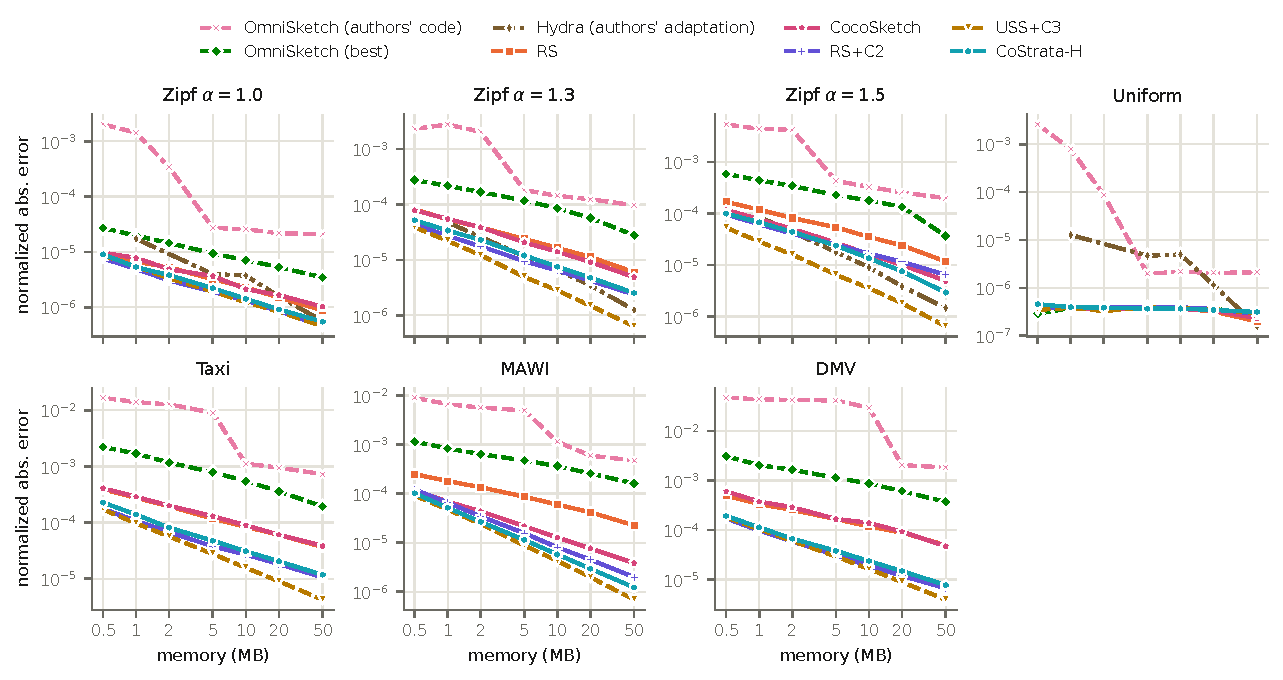
\includegraphics[width=\textwidth]{figs/nae_vs_mem.pdf}
\caption{Normalized absolute error on record-sampled queries with $k\ge2$ predicates versus memory
(mean of 5 seeds; lower is better). ``\omni (best cfg.)'' is the best of eight configurations under
oracle memory accounting, chosen separately for every point.}
\label{fig:nae}
\end{figure}

\begin{table}[t]
\centering\small
\caption{Normalized absolute error, record-sampled queries with $k\ge2$ predicates (mean of 5 seeds).
Bold: best method per column and budget.}
\label{tab:main}
\begin{tabular}{lrrrrrr}
\toprule
Method & Zipf $\alpha{=}1.0$ & Zipf $\alpha{=}1.3$ & Zipf $\alpha{=}1.5$ & Uniform & Taxi & MAWI \\
\midrule
\multicolumn{7}{l}{\emph{1 MB}} \\
OmniSketch {\footnotesize(paper)} & 3.4e-5 & 3.7e-4 & 8.1e-4 & 1.7e-6 & 2.7e-3 & 1.5e-3 \\
OmniSketch {\footnotesize(best cfg.)} & 2.1e-5 & 2.2e-4 & 4.4e-4 & \textbf{3.8e-7} & 1.8e-3 & 8.3e-4 \\
Reservoir {\footnotesize(RS)} & \textbf{6.7e-6} & 5.4e-5 & 1.2e-4 & 4.0e-7 & 2.7e-4 & 1.8e-4 \\
USS & 8.2e-6 & 5.9e-5 & 7.9e-5 & 4.2e-7 & 3.1e-4 & 6.0e-5 \\
RS+C & 7.7e-6 & 6.2e-5 & 1.3e-4 & 4.1e-7 & 2.2e-4 & 1.1e-4 \\
USS+C & 7.6e-6 & \textbf{5.3e-5} & \textbf{7.7e-5} & 4.2e-7 & \textbf{2.1e-4} & \textbf{5.9e-5} \\
CoStrata & 8.0e-6 & 7.5e-5 & 1.7e-4 & 4.1e-7 & 2.6e-4 & 1.2e-4 \\
\midrule
\multicolumn{7}{l}{\emph{10 MB}} \\
OmniSketch {\footnotesize(paper)} & 2.0e-5 & 1.6e-4 & 3.1e-4 & 1.4e-6 & 1.4e-3 & 6.0e-4 \\
OmniSketch {\footnotesize(best cfg.)} & 8.4e-6 & 1.0e-4 & 1.8e-4 & 3.8e-7 & 5.6e-4 & 3.8e-4 \\
Reservoir {\footnotesize(RS)} & \textbf{2.3e-6} & 1.6e-5 & 3.5e-5 & \textbf{3.7e-7} & 8.4e-5 & 5.9e-5 \\
USS & 2.5e-6 & 1.5e-5 & \textbf{1.7e-5} & 3.8e-7 & 9.4e-5 & 1.1e-5 \\
RS+C & 2.8e-6 & 1.9e-5 & 3.9e-5 & 3.9e-7 & 7.4e-5 & 2.7e-5 \\
USS+C & 2.6e-6 & \textbf{1.4e-5} & 1.8e-5 & 3.8e-7 & \textbf{6.5e-5} & \textbf{1.0e-5} \\
CoStrata & 2.9e-6 & 2.3e-5 & 5.0e-5 & 3.9e-7 & 8.2e-5 & 2.8e-5 \\
\bottomrule
\end{tabular}

\end{table}

\paragraph{Sanity check of the \omni re-implementation.} For three-predicate queries at 10\,MB---the
setting of Fig.~6 of~\cite{omni}---our implementation with the paper's parameters yields an NAE of
\NumOmniPaperKthreeZipfTen, \NumOmniPaperKthreeZipfThirteen{} and \NumOmniPaperKthreeZipfFifteen{} on the
Zipf streams with $\alpha=1.0, 1.3, 1.5$ and \NumOmniPaperKthreeUnif{} on the uniform stream. The
original figure shows the same qualitative picture (an error close to zero for the uniform stream that
grows with $\alpha$ to a few $10^{-4}$); an exact match cannot be expected because hash functions and
query samples differ.

\paragraph{Row sampling versus \omni.} Figure~\ref{fig:nae} and Table~\ref{tab:main} show the main
result. Across all six streams and seven budgets, the row reservoir has a
\NumOmniPaperVsResLo--\NumOmniPaperVsResHi$\times$ lower error than \omni with the published
parameters (geometric mean \NumOmniPaperVsResGm$\times$). Tuning does not close the gap: on the five
non-uniform streams, the best of the eight \omni configurations under oracle accounting is still
\NumOmniBestVsResLo--\NumOmniBestVsResHi$\times$ worse than the reservoir (geometric mean
\NumOmniBestVsResGm$\times$). The only tie is the Uniform stream, where multi-predicate queries match one or
two records, every method essentially returns zero, and the ratio is
\NumOmniBestVsResUnifLo--\NumOmniBestVsResUnifHi. Including single-predicate queries makes the published
configuration look worse (\NumOmniPaperVsResAllLo--\NumOmniPaperVsResAllHi$\times$, geometric mean
\NumOmniPaperVsResAllGm$\times$), because with $w=8$ columns it is a very coarse Count-Min sketch.
The shape of the curves confirms the analysis of Section~\ref{sec:anatomy}: the error of every
sample-based synopsis falls roughly as $M^{-1/2}$, whereas that of \omni (paper) flattens---on the
Uniform stream it stays between $\NumOmniPaperFlatLo\cdot10^{-6}$ and $\NumOmniPaperFlatHi\cdot10^{-6}$
over a hundred-fold increase in memory---because the collision term of
Proposition~\ref{prop:bias} does not depend on $B$. No single configuration wins the search: the published $(w,d)=(8,3)$ with lean accounting or $(64,2)$ is best
at small and medium budgets, and $(4096,1)$ at the largest ones, i.e., large budgets are better spent on
width than on ever larger per-cell samples.

\begin{table}[t]
\centering\footnotesize\setlength{\tabcolsep}{3.5pt}
\caption{NAE by number of predicates $k$ at 10\,MB, record-sampled queries (mean of 5 seeds).}
\label{tab:byk}
\begin{tabular}{lrrrrrrrrrrrr}
\toprule
 & \multicolumn{6}{c}{Taxi, number of predicates $k$} & \multicolumn{6}{c}{MAWI, number of predicates $k$} \\
Method & 1 & 2 & 3 & 4 & 5 & 6 & 1 & 2 & 3 & 4 & 5 & 6 \\
\midrule
Omni. (paper) & 3.2e-3 & 4.1e-3 & 2.1e-3 & 7.3e-4 & 1.6e-4 & 6.9e-5 & 2.3e-3 & 1.4e-3 & 7.5e-4 & 3.3e-4 & 2.6e-4 & 2.6e-4 \\
Omni. (best cfg.) & 1.7e-5 & 1.3e-3 & 9.5e-4 & 4.0e-4 & 9.4e-5 & 4.7e-5 & 8.7e-5 & 7.6e-4 & 4.5e-4 & 1.6e-4 & 1.4e-4 & 1.4e-4 \\
RS & 2.7e-4 & 2.1e-4 & 1.3e-4 & \textbf{5.0e-5} & \textbf{1.6e-5} & \textbf{8.3e-6} & 1.4e-4 & 1.1e-4 & 7.9e-5 & 3.9e-5 & 3.3e-5 & 3.1e-5 \\
USS & 3.0e-4 & 2.3e-4 & 1.5e-4 & 6.1e-5 & 1.8e-5 & 8.9e-6 & 5.4e-5 & 2.8e-5 & 1.9e-5 & \textbf{4.4e-6} & \textbf{3.5e-6} & \textbf{1.6e-6} \\
RS+C & 3.9e-6 & 1.6e-4 & 1.2e-4 & 5.8e-5 & 1.8e-5 & 1.0e-5 & 6.8e-6 & 5.3e-5 & 3.7e-5 & 1.7e-5 & 1.5e-5 & 1.1e-5 \\
USS+C & \textbf{1.8e-6} & \textbf{1.4e-4} & \textbf{1.1e-4} & 5.1e-5 & 1.7e-5 & 8.4e-6 & \textbf{2.9e-6} & \textbf{2.3e-5} & \textbf{1.5e-5} & 5.5e-6 & 4.9e-6 & 3.6e-6 \\
CoStrata & 4.3e-6 & 1.8e-4 & 1.4e-4 & 6.3e-5 & 2.0e-5 & 1.1e-5 & 7.1e-6 & 5.4e-5 & 4.0e-5 & 1.9e-5 & 1.6e-5 & 1.3e-5 \\
\bottomrule
\end{tabular}

\end{table}

\paragraph{Calibration.} Table~\ref{tab:byk} breaks the error down by the number of predicates. For
$k=1$ the calibrated synopses (\textsc{RS+C}, \textsc{USS+C}, \cs) are one to two orders of magnitude more
accurate than the uncalibrated samples, simply because the estimate is tied to an exact counter of a
fine-grained bucket. This is where most of the overall gain of calibration comes from: over all $k$,
\textsc{RS+C} improves on RS by a geometric mean of \NumCalibRsAllGm$\times$
(\NumCalibRsAllLo--\NumCalibRsAllHi$\times$) and \textsc{USS+C} on USS by \NumCalibUssAllGm$\times$. For
$k\ge2$ the picture is mixed and data dependent: calibration helps on MAWI
(\NumCalibRsMawiLo--\NumCalibRsMawiHi$\times$), where attributes are strongly correlated and a query
often covers most of its lightest bucket, helps slightly on Taxi
(\NumCalibRsTaxiLo--\NumCalibRsTaxiHi$\times$), and \emph{hurts} on the synthetic streams with independent
attributes (\NumCalibRsSynLo--\NumCalibRsSynHi$\times$, geometric mean \NumCalibRsSynGm$\times$), where the
marginal count carries little information about a conjunction and the calibrated sample simply holds fewer
rows (it pays for the counters, a 64-bit priority per row, and compaction slack). Over all streams the
geometric-mean gain for $k\ge2$ is \NumCalibRsGm$\times$.

\paragraph{USS.} Where full tuples repeat, aggregating them pays off: on MAWI (25\% distinct tuples) USS is
\NumUssVsResMawiLo--\NumUssVsResMawiHi$\times$ more accurate than the reservoir and, with calibration,
the most accurate method overall; the same holds, to a lesser degree, for the Zipf stream with
$\alpha=1.5$ (49\% distinct tuples). On Taxi (97\% distinct tuples) USS is slightly worse than the reservoir
because of its per-entry overhead. Across the board, \textsc{USS+C} is the best or close to the best
method in Table~\ref{tab:main}.

\paragraph{\cs on frequent queries.} On this workload, which is dominated by frequent values, \cs is
\NumCsVsRscLo--\NumCsVsRscHi$\times$ (geometric mean \NumCsVsRscGm$\times$) less accurate than the calibrated
uniform sample \textsc{RS+C}: this is the price of reserving half of the nominal budget for the hash
strata, and it stays well within the $\sqrt2$ bound of Proposition~\ref{prop:size}. Relative to the plain
reservoir \cs ranges from $1/\NumCsVsResLo\approx2\times$ better (MAWI) to \NumCsVsResHi$\times$ worse
(Zipf streams), with a geometric mean of \NumCsVsResGm. \cs is therefore not a better
general-purpose estimator for frequent conjunctions; its purpose is the regime discussed next.

\subsection{Rare anchors: when stratification pays}\label{sec:anchor}

\begin{figure}[t]
\centering
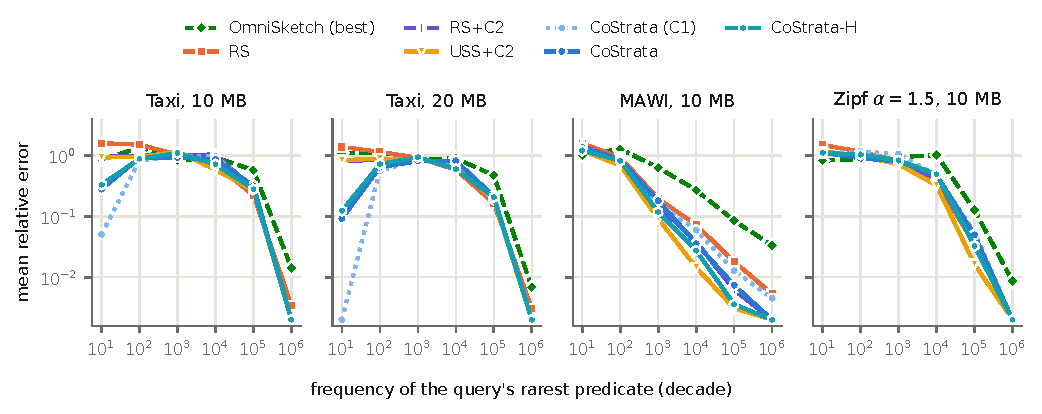
\includegraphics[width=\textwidth]{figs/anchor.pdf}
\caption{Mean relative error of anchored queries, grouped by the frequency decade of the rarest
predicate (mean of 5 seeds). Values near 1 mean that the synopsis has essentially no information about
the query.}
\label{fig:anchor}
\end{figure}

Figure~\ref{fig:anchor} groups anchored queries by the frequency of their rarest predicate.
On Taxi, whose attributes have between 4 and 697 distinct values, most values own a bucket, and \cs
guarantees each of them about $B$ sampled rows. For anchors that occur 10--99 times, the mean relative
error of \cs is \NumTaxiDOneCsFive{} at 5\,MB, \NumTaxiDOneCsTen{} at 10\,MB and \NumTaxiDOneCsTwenty{} at
20\,MB, while the best competitor stays at \NumTaxiDOneOtherFive, \NumTaxiDOneOtherTen{} and
\NumTaxiDOneOtherTwenty, respectively---an improvement of \NumTaxiDOneGainFive$\times$,
\NumTaxiDOneGainTen$\times$ and more than two orders of magnitude; at 50\,MB all such queries are answered
essentially exactly, as predicted by Proposition~\ref{prop:rare} (the automatic $B$ exceeds the bucket
counts). For anchors occurring 100--999 times the gain is \NumTaxiDTwoGainTen$\times$ at 10\,MB and
\NumTaxiDTwoGainFifty$\times$ at 50\,MB. The effect needs a sufficient budget: at 1\,MB, $B\approx5$ and \cs
is indistinguishable from \textsc{RS+C}. For frequent anchors ($10^4$--$10^6$ occurrences) the relative error of \cs is
\NumTaxiFreqPenaltyLo--\NumTaxiFreqPenaltyHi$\times$ that of the reservoir, which again reflects its smaller
uniform share.

On MAWI and on the Zipf streams, stratification is neutral: the strata of IP addresses, ports, or of a
10\,000-value Zipf domain are all of comparable weight, and with tens of thousands of non-empty buckets
$B$ is between 2 and 30 rows, so the house stratum dominates. Here the ranking is determined by
calibration and, on MAWI, by tuple aggregation (USS and \textsc{USS+C} are best in every decade).
\omni does not benefit from its per-cell samples in either case: for rare anchors its relative error
is close to or above 1 for every configuration, because the usable rate is that of the heaviest cell
(Observation~\ref{obs:min}) and collisions inflate small counts.

\subsection{Update throughput and query latency}\label{sec:speed}

\begin{table}[t]
\centering\small
\caption{Update throughput and query latency on one core (median of 3 runs). Latency is the mean over the
2\,400 queries of the workload, after a one-time preparation pass (sorting cells for \omni, computing
weights for \cs).}
\label{tab:speed}
\begin{tabular}{lrrrrrr}
\toprule
 & \multicolumn{3}{c}{Taxi ($p{=}12$)} & \multicolumn{3}{c}{MAWI ($p{=}10$)} \\
Method & 1 MB & 10 MB & 50 MB & 1 MB & 10 MB & 50 MB \\
\midrule
\multicolumn{7}{l}{\emph{Update throughput (million records/s)}} \\
RS & 520.7 & -- & -- & -- & -- & -- \\
USS & 17.5 & -- & -- & -- & -- & -- \\
RS+C1 & 32.2 & -- & -- & -- & -- & -- \\
RS+C2 & 5.2 & -- & -- & -- & -- & -- \\
USS+C2 & 4.2 & -- & -- & -- & -- & -- \\
aSH & 3.2 & -- & -- & -- & -- & -- \\
OmniSketch (port of authors' code) & 13.7 & -- & -- & -- & -- & -- \\
OmniSketch (ours, same $B$) & 12.0 & -- & -- & -- & -- & -- \\
OmniSketch (journal cfg.) & 11.2 & -- & -- & -- & -- & -- \\
OmniSketch ($8{\times}3$, lean) & 10.5 & -- & -- & -- & -- & -- \\
OmniSketch ($256{\times}2$) & 14.2 & -- & -- & -- & -- & -- \\
OmniSketch ($1024{\times}2$) & 10.7 & -- & -- & -- & -- & -- \\
\midrule
\multicolumn{7}{l}{\emph{Query latency ($\mu$s per query)}} \\
RS & 22 & 229 & 1273 & 22 & 231 & 1274 \\
USS & 29 & 350 & 2821 & 28 & 328 & 2594 \\
OmniSketch (ours, same $B$) & 3.7 & 20 & 96 & 2.9 & 25 & 121 \\
OmniSketch ($256{\times}2$) & 1.0 & 9.5 & 68 & 0.6 & 4.5 & 22 \\
OmniSketch ($1024{\times}2$) & 0.6 & 7.1 & 52 & 0.2 & 1.3 & 5.5 \\
\bottomrule
\end{tabular}

\end{table}

Table~\ref{tab:speed} reports single-core performance. The reservoir is in a class of its own
(\NumTpResLo--\NumTpResHi{} million records/s) because skip counting touches only sampled records.
\cs ingests \NumTpCsLo--\NumTpCsHi{} million records/s: its per-record cost is $p$ hash evaluations and
counter increments, plus compactions, which become noticeable when the sample is a large fraction of the
stream (50\,MB is 11\% of Taxi). It is \NumTpCsVsOmniLo--\NumTpCsVsOmniHi$\times$ faster than the fastest
\omni configuration at every budget and at least as fast as USS, which must probe a hash table and update a
heap for every record. Our \omni re-implementation reaches
\NumTpOmniPaperLo--\NumTpOmniPaperHi{} million records/s with the published parameters; the original Java
implementation is reported at 0.09--0.2 million records/s on different hardware~\cite{omni}, so the
flat-heap and threshold-array engineering of Section~\ref{sec:setup} matters, and our accuracy
comparison is not against a slow strawman. With lean accounting the same budget buys four times
larger samples, and throughput drops to \NumTpOmniLeanLo{} million records/s at 50\,MB because heaps of
tens of thousands of entries are updated for a large part of the stream.

Query latency is the one dimension in which \omni is clearly ahead, at every budget: it merges $|Q|\,d$
sorted lists of at most $B$ hashes (\NumQlatOmniLo--\NumQlatOmniHi\,$\mu$s per query), whereas the row
samples scan the first predicate's column over the whole sample (\NumQlatCsLo--\NumQlatCsHi\,$\mu$s for \cs,
i.e., \NumQlatCsVsOmniPaperLo--\NumQlatCsVsOmniPaperHi$\times$ slower than \omni with the published parameters
and up to \NumQlatCsVsOmniHi$\times$ slower than its fastest configuration). \cs is somewhat faster than the
reservoir and USS because it holds fewer rows. For workloads with many queries per synopsis a per-bucket index on the row store would
make selective predicates sub-linear; we leave this to future work.

\subsection{Scaling the number of attributes}\label{sec:census}

\begin{figure}[t]
\centering
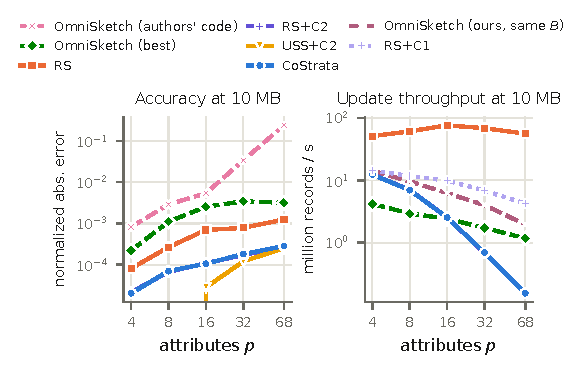
\includegraphics[width=\textwidth]{figs/census_scaling.pdf}
\caption{Census stream restricted to its first $p$ attributes, 10\,MB (accuracy: mean of 3 seeds;
throughput: one core, with $(w,d)=(256,2)$ for the ``best cfg.'' series).}
\label{fig:census}
\end{figure}

The main argument for \omni over Hydra is linear scaling in $p$. Row samples scale the same way---a row
costs $p$ words---and Figure~\ref{fig:census} shows that the accuracy ranking is unchanged from 4 to 68
attributes: at $p=68$ the reservoir is \NumCensusOmniBestVsResSixtyEight$\times$ more accurate than the
best \omni configuration, and \cs another \NumCensusResVsCsSixtyEight$\times$ more accurate than the
reservoir (Census attributes are correlated categorical variables, the favourable case for
calibration). For small $p$ the stream has few distinct tuples and USS is nearly exact; its advantage
shrinks as $p$ grows and has vanished at $p=68$. Throughput at $p=68$ is \NumCensusTpCsSixtyEight{} million
records/s for \cs and \NumCensusTpOmniSixtyEight{} for \omni (paper parameters).

\subsection{Ablations and estimator validity}\label{sec:ablation}

\begin{table}[t]
\centering\small
\caption{\cs design space at 10\,MB (mean of 5 seeds): NAE on record-sampled queries with $k\ge2$, and
mean relative error of anchored queries whose rarest predicate occurs 10--99 and 100--999 times.}
\label{tab:ablation}
\begin{tabular}{lrrrrrr}
\toprule
 & \multicolumn{3}{c}{Taxi} & \multicolumn{3}{c}{MAWI} \\
Variant & NAE & anchor $10^1$ & anchor $10^2$ & NAE & anchor $10^1$ & anchor $10^2$ \\
\midrule
\multicolumn{7}{l}{\emph{pair-table share} $\phi_2$ \emph{(uniform sample)}} \\
\quad none (RS+C1) & 7.2e-5 & 1.2 & 1.2 & 2.5e-5 & 1.4 & 0.84 \\
\quad $\phi_2=0.05$ & 2.9e-5 & 1.1 & 1.1 & 1.2e-5 & 1.4 & 0.85 \\
\quad $\phi_2=0.1$ & 2.7e-5 & 1.1 & 1.1 & 9.8e-6 & 1.4 & 0.89 \\
\quad $\phi_2=0.25$ (default) & 2.7e-5 & 0.94 & 1 & 8.0e-6 & 1.4 & 0.85 \\
\quad $\phi_2=0.5$ & 3.1e-5 & 0.94 & 0.8 & 7.1e-6 & 1.3 & 0.84 \\
\multicolumn{7}{l}{\emph{pair and triple tables} $\phi_2/\phi_3$} \\
\quad $0.1/0.1$ & 1.8e-5 & 1.1 & 1.1 & 9.6e-6 & 1.5 & 0.89 \\
\quad $0.15/0.15$ (RS+C3) & 1.7e-5 & 1 & 1.1 & 8.0e-6 & 1.4 & 0.88 \\
\quad $0.2/0.3$ & 1.5e-5 & 0.98 & 1 & 8.2e-6 & 1.4 & 0.96 \\
\multicolumn{7}{l}{\emph{all anchors (raking) instead of the lightest}} \\
\quad $\phi_2=0.25$, all anchors & 2.2e-5 & 1.1 & 1.2 & 1.1e-5 & 1.5 & 0.94 \\
\quad $0.15/0.15$, all anchors & 1.9e-5 & 1.4 & 1.3 & 1.8e-5 & 1.6 & 1 \\
\multicolumn{7}{l}{\emph{house weight} $\lambda$ \emph{(C1 only)}} \\
\quad $\lambda=0$ (strata only) & 1.9e-4 & 0.002 & 0.26 & 9.5e-5 & 1.2 & 0.83 \\
\quad $\lambda=1/4$ & 9.2e-5 & 0.0065 & 0.48 & 3.6e-5 & 1.3 & 0.86 \\
\quad $\lambda=1$ & 7.8e-5 & 0.051 & 0.83 & 2.6e-5 & 1.4 & 0.85 \\
\quad $\lambda=4$ & 7.3e-5 & 0.45 & 0.99 & 2.6e-5 & 1.4 & 0.85 \\
\multicolumn{7}{l}{\emph{house weight with pair tables}} \\
\quad $\lambda=1/4$, $\phi_2=0.25$ & 3.2e-5 & 0.12 & 0.68 & 1.0e-5 & 1.2 & 0.8 \\
\quad $\lambda=1$, $\phi_2=0.25$ (\cs) & 2.8e-5 & 0.28 & 0.92 & 8.5e-6 & 1.4 & 0.87 \\
\multicolumn{7}{l}{\emph{hold mode (}$\phi_2=0.25$\emph{)}} \\
\quad $\lambda=1/4$ & 3.8e-5 & 0.1 & 0.79 & 7.9e-6 & 1.2 & 0.8 \\
\quad $\lambda=1$ (\csh) & 3.1e-5 & 0.33 & 0.89 & 5.7e-6 & 1.2 & 0.82 \\
\quad $\lambda=4$ & 2.8e-5 & 0.59 & 0.79 & 5.0e-6 & 1.4 & 0.76 \\
\quad USS+C2 (no strata) & 2.6e-5 & 0.93 & 0.95 & 4.2e-6 & 1.2 & 0.69 \\
\multicolumn{7}{l}{\emph{allocation exponent} $\gamma$ \emph{(}$\lambda=0$\emph{, C1 only)}} \\
\quad $\gamma=0.75$ & 1.3e-4 & 0.0065 & 0.46 & 5.3e-5 & 1.2 & 0.81 \\
\quad $\gamma=0.5$ & 9.4e-5 & 0.32 & 0.81 & 3.5e-5 & 1.3 & 0.78 \\
\multicolumn{7}{l}{\emph{buckets per attribute} $w$ \emph{(}$\lambda=1$\emph{, C1 only)}} \\
\quad $w=64$ & 8.1e-5 & 0.83 & 1.1 & 4.7e-5 & 1.4 & 0.88 \\
\quad $w=256$ & 7.9e-5 & 0.4 & 0.84 & 4.0e-5 & 1.3 & 0.88 \\
\quad $w=1024$ & 7.8e-5 & 0.13 & 0.87 & 3.3e-5 & 1.3 & 0.86 \\
\quad $w=4096$ & 7.7e-5 & 0.052 & 0.81 & 2.8e-5 & 1.4 & 0.9 \\
\quad $w=16384$ & 8.1e-5 & 0.054 & 0.84 & 2.7e-5 & 1.3 & 0.86 \\
\multicolumn{7}{l}{\emph{reference}} \\
\quad RS & 8.4e-5 & 1.6 & 1.5 & 5.9e-5 & 1.6 & 0.94 \\
\bottomrule
\end{tabular}

\end{table}

\paragraph{House weight and allocation.} Table~\ref{tab:ablation} varies one design choice at a time.
The house weight $\lambda$ trades accuracy on frequent queries against accuracy on rare anchors exactly
as intended: without a house stratum ($\lambda=0$) rare anchors on Taxi are answered almost exactly but
the NAE is 2.5 times that of the reservoir; $\lambda=1$ gives up some of the rare-anchor gain and matches
the reservoir's NAE; $\lambda=1/4$ is a reasonable alternative when rare values matter most. A
sub-linear allocation exponent $\gamma<1$ without a house stratum is dominated by $\gamma=1$ with a
house stratum (compare $\gamma=0.5$ with $\lambda=1/4$: same NAE, 50 times larger error on rare anchors).
On MAWI none of these choices matters much for rare anchors, in line with Section~\ref{sec:anchor}.

\paragraph{Number of buckets.} On Taxi, rare-anchor accuracy improves until every value owns a bucket
($w\approx4096$) and is flat afterwards; on MAWI, larger $w$ improves the NAE because finer buckets make
calibration sharper. The automatic rule (5\% of the budget for counters) selects $w=8192$ at 10\,MB.

\paragraph{Calibrated versus Horvitz--Thompson estimates.} Over all record-sampled queries at 10\,MB, the
calibrated estimate of \cs has a \NumHtVsCalTaxi$\times$ (Taxi), \NumHtVsCalMawi$\times$ (MAWI) and
\NumHtVsCalZipf$\times$ (Zipf, $\alpha=1.5$) lower NAE than its HT estimate from the same sample.

\paragraph{Unbiasedness.} To check Theorem~\ref{thm:unbiased} empirically we ran \cs with many additional
independent seeds at budgets at which compactions are frequent: \NumBiasSeedsTaxi{} seeds on Taxi (1\,MB)
and \NumBiasSeedsZipf{} seeds on Zipf $\alpha=1.5$ (0.5\,MB). Summed over the queries with $f(q)\ge1000$, the HT
estimates deviate from the truth by $\NumBiasHtTotalTaxi\%\pm\NumBiasHtTotalSeTaxi\%$ (Taxi) and
$\NumBiasHtTotalZipf\%\pm\NumBiasHtTotalSeZipf\%$ (Zipf; mean $\pm$ standard error over seeds), and
\NumBiasHtZTaxi\% and \NumBiasHtZZipf\% of the per-query $z$-scores of the seed-averaged estimates lie within
$\pm1.96$. (For transparency: a first batch of 300 seeds on Taxi showed $+0.15\%\pm0.06\%$; we then added
900 seeds, which on their own give $+0.01\%\pm0.03\%$; the numbers above pool both batches.) The
calibrated estimator, a ratio estimator, deviates by
$\NumBiasCalTotalTaxi\%\pm\NumBiasCalTotalSeTaxi\%$ and $\NumBiasCalTotalZipf\%\pm\NumBiasCalTotalSeZipf\%$.

\begin{table}[t]
\centering\small
\caption{Coverage (\%) of nominal 95\% intervals $\hat f_{\mathrm C}\pm1.96\sqrt{\hat V_{\mathrm C}}$ of \cs,
over all queries and over queries with $f(q)\ge100$.}
\label{tab:cov}
\begin{tabular}{llrrrrrrr}
\toprule
 & & \multicolumn{3}{c}{normal approx.} & \multicolumn{4}{c}{rule of three / gamma} \\
\cmidrule(lr){3-5}\cmidrule(lr){6-9}
Method & MB & all & $f{<}100$ & $f{\ge}100$ & all & $f{<}100$ & $f{\ge}100$ & $m{=}0$ \\
\midrule
\cs & 0.5 & 31 & 3 & 70 & 94 & 99 & 88 & 100 \\
 & 1 & 34 & 5 & 75 & 92 & 98 & 85 & 100 \\
 & 10 & 49 & 22 & 88 & 93 & 96 & 89 & 100 \\
 & 50 & 64 & 47 & 91 & 92 & 93 & 92 & 100 \\
\addlinespace[2pt]
RS+C2 & 0.5 & 31 & 2 & 71 & 94 & 99 & 89 & 100 \\
 & 1 & 34 & 3 & 76 & 93 & 99 & 86 & 100 \\
 & 10 & 47 & 17 & 89 & 93 & 96 & 90 & 100 \\
 & 50 & 59 & 38 & 91 & 92 & 93 & 91 & 100 \\
\addlinespace[2pt]
\csh & 0.5 & 30 & 3 & 66 & 93 & 99 & 87 & 100 \\
 & 1 & 33 & 5 & 73 & 92 & 98 & 85 & 100 \\
 & 10 & 48 & 22 & 88 & 93 & 96 & 90 & 100 \\
 & 50 & 63 & 46 & 93 & 93 & 93 & 93 & 100 \\
\bottomrule
\end{tabular}

\end{table}

\paragraph{Confidence intervals: a caveat.} The plug-in variance estimate~\eqref{eq:cal} should not be
used blindly. Table~\ref{tab:cov} shows that normal-approximation intervals reach close to nominal
coverage only when the query has enough sampled matches (large budgets, $f(q)\ge100$); for small
budgets and for rare queries coverage is far below 95\%, mainly because a query without any sampled match
receives the degenerate interval $[0,0]$. Reliable intervals for small counts would need a
different construction (e.g., based on the retention probability of the lightest bucket), which we have
not developed.


\section{Related Work}\label{sec:related}

\paragraph{Synopses for ad-hoc predicates on streams.} Hydra~\cite{hydra} hashes each record into a
sketch of universal sketches~\cite{univmon} once per attribute subset and is exponential in $p$.
\omni~\cite{omni,omni-sr} replaced this by per-attribute sketches with embedded samples; its journal
version~\cite{omni-vldbj} extends it to bounded deletions and compares it with adaptive
sample-and-hold~\cite{ash} in that model, which is outside the scope of our insert-only study.
We are not aware of a prior comparison of \omni with row sampling or with multi-objective samples.
In network measurement, CocoSketch~\cite{coco} answers arbitrary partial-key queries from a table of
full keys maintained with unbiased replacement, close in spirit to USS~\cite{ting-uss}.

\paragraph{Coordinated and multi-objective sampling.} Bottom-$k$ and priority
sampling~\cite{bottomk,priority} underlie both \omni's cells and our budget control. The principle that
the union of coordinated samples serves every objective with the maximum inclusion probability is due
to Cohen~\cite{cohen-mo}; Ting~\cite{ting-ats} unifies adaptive thresholds and outlines multi-stratified
sampling with per-stratum bottom-$k$ thresholds. \cs is an engineered instance of this principle for
ad-hoc predicates over many attributes: strata are hashed (domains are unknown and unbounded), thresholds
are counter-driven (no per-stratum priority structure), the budget is a single scalar, and a house
stratum bounds the loss against uniform sampling. Congressional samples~\cite{congress}, small-group
sampling~\cite{smallgroup}, CVOPT~\cite{cvopt} and S-VOILA~\cite{svoila} address stratified sampling
for group-by queries with known grouping attributes or a single stratification.

\paragraph{Calibration.} Using known totals to improve sample-based estimates is classical in survey
sampling~\cite{sarndal,calibration}; AQP\texttt{++}~\cite{aqppp} combines samples with precomputed
aggregates in a database setting. Our contribution is the observation that a depth-one Count-Min row
per attribute---state that the stratified sampler needs anyway---is an effective source of such
totals for conjunctive queries on streams.

\section{Discussion and Limitations}\label{sec:discussion}

\emph{Scope of the negative result.} Our claim concerns \textsc{count} queries with conjunctive
predicates in the insert-only model, for attribute values that fit a machine word (or a fingerprint,
which suffices for equality predicates). We did not study deletions; row samples do not survive
arbitrary deletions, and the bounded-deletion variant of \omni~\cite{omni-vldbj} deserves a separate
comparison against deletion-aware samplers~\cite{ash}. \emph{Where \cs does not help.} Equal
allocation per stratum can only lift strata whose total mass is small; for attributes whose tail
carries a large share of the stream (IP addresses, ports), hashed strata are all of similar weight
and \cs behaves like a calibrated uniform sample. When full tuples repeat frequently, row-level
sampling wastes memory on duplicates and USS is the better base synopsis; making \cs
tuple-aggregating is future work. \emph{Query latency.} Row samples are scanned linearly, whereas
\omni intersects $|Q|d$ sorted lists and answers one to two orders of magnitude faster
(Section~\ref{sec:speed}). Per-stratum indexes on the row store would close this gap.
\emph{Threats to validity.} We could not run on the SNMP and CAIDA traces of~\cite{omni} and
re-implemented \omni rather than using the Java code; we mitigate this by reproducing the synthetic
setting of~\cite{omni}, where our implementation shows the reported error pattern, and by giving
\omni a configuration search and oracle accounting that it would not have in practice. All experiments
ran on a single laptop CPU; absolute throughputs will differ on server hardware.

\section{Conclusion}

For predicate counting over multi-attribute streams, the sketch-in-sketch design of \omni is dominated
at equal memory by a plain sample of rows, and the reason is structural: coordinated per-cell samples
of record identifiers can only be combined by intersection, which yields the rate of the heaviest
stratum, while every sampled record is paid for once per attribute and row. Turning the coordination
around---storing rows once and keeping a row if any of its strata would keep it---realises the benefit
of hash stratification, and the counters that drive the thresholds double as calibration totals. The
resulting synopsis, \cs, is simple (a counter row per attribute, a row store, one scalar), unbiased,
mergeable, and fast; its accuracy advantage, however, is confined to queries anchored on rare values of
attributes whose tail carries little mass, and for frequent conjunctions a (calibrated) uniform or
tuple-aggregating sample remains the method of choice. More broadly, our study suggests that composite sketches whose cells contain
\emph{samples} should be evaluated against the corresponding global sampling design under a careful,
shared memory accounting.

\paragraph{Reproducibility.} The code of all synopses, the dataset converters, the workload generator
and the scripts that produce every figure and table of this paper are included in the accompanying
repository.

\begin{thebibliography}{99}\small
\bibitem{birdseye} M.~Garofalakis. A bird's-eye view of complex streaming data analytics. In \emph{Proc.\ DEBS}, 2025. doi:10.1145/3701717.3733848.
\bibitem{synopses} G.~Cormode, M.~Garofalakis, P.~J. Haas, and C.~Jermaine. Synopses for massive data: Samples, histograms, wavelets, sketches. \emph{Foundations and Trends in Databases}, 4(1--3):1--294, 2012.
\bibitem{omni} W.~R. Punter, O.~Papapetrou, and M.~Garofalakis. OmniSketch: Efficient multi-dimensional high-velocity stream analytics with arbitrary predicates. \emph{PVLDB}, 17(3):319--331, 2023.
\bibitem{omni-sr} W.~R. Punter, O.~Papapetrou, and M.~Garofalakis. OmniSketch: Streaming data analytics with arbitrary predicates. \emph{SIGMOD Record}, 54(1):28--35, 2025.
\bibitem{omni-vldbj} W.~R. Punter, O.~Papapetrou, and M.~Garofalakis. OmniSketch: Multi-dimensional update stream analytics with arbitrary predicates. \emph{The VLDB Journal}, 2026. doi:10.1007/s00778-025-00960-6.
\bibitem{hydra} A.~Manousis, Z.~Cheng, R.~Ben~Basat, Z.~Liu, and V.~Sekar. Enabling efficient and general subpopulation analytics in multidimensional data streams. \emph{PVLDB}, 15(11):3249--3262, 2022.
\bibitem{ecm} O.~Papapetrou, M.~Garofalakis, and A.~Deligiannakis. Sketch-based querying of distributed sliding-window data streams. \emph{PVLDB}, 5(10):992--1003, 2012.
\bibitem{ting-mdc} D.~Ting. Approximate distinct counts for billions of datasets. In \emph{Proc.\ SIGMOD}, 2019.
\bibitem{cm} G.~Cormode and S.~Muthukrishnan. An improved data stream summary: The count-min sketch and its applications. \emph{Journal of Algorithms}, 55(1):58--75, 2005.
\bibitem{pagh} R.~Pagh, M.~St\"ockel, and D.~P. Woodruff. Is min-wise hashing optimal for summarizing set intersection? In \emph{Proc.\ PODS}, pages 109--120, 2014.
\bibitem{vitter} J.~S. Vitter. Random sampling with a reservoir. \emph{ACM Transactions on Mathematical Software}, 11(1):37--57, 1985.
\bibitem{li} K.-H. Li. Reservoir-sampling algorithms of time complexity $O(n(1+\log(N/n)))$. \emph{ACM Transactions on Mathematical Software}, 20(4):481--493, 1994.
\bibitem{ht} D.~G. Horvitz and D.~J. Thompson. A generalization of sampling without replacement from a finite universe. \emph{Journal of the American Statistical Association}, 47(260):663--685, 1952.
\bibitem{bottomk} E.~Cohen and H.~Kaplan. Summarizing data using bottom-k sketches. In \emph{Proc.\ PODC}, pages 225--234, 2007.
\bibitem{priority} N.~Duffield, C.~Lund, and M.~Thorup. Priority sampling for estimation of arbitrary subset sums. \emph{Journal of the ACM}, 54(6), 2007.
\bibitem{cohen-mo} E.~Cohen. Multi-objective weighted sampling. In \emph{Proc.\ HotWeb}, 2015. Full version: arXiv:1509.07445.
\bibitem{ting-ats} D.~Ting. Adaptive threshold sampling. In \emph{Proc.\ SIGMOD}, 2022. arXiv:1708.04970.
\bibitem{ting-uss} D.~Ting. Data sketches for disaggregated subset sum and frequent item estimation. In \emph{Proc.\ SIGMOD}, 2018.
\bibitem{congress} S.~Acharya, P.~B. Gibbons, and V.~Poosala. Congressional samples for approximate answering of group-by queries. In \emph{Proc.\ SIGMOD}, pages 487--498, 2000.
\bibitem{smallgroup} B.~Babcock, S.~Chaudhuri, and G.~Das. Dynamic sample selection for approximate query processing. In \emph{Proc.\ SIGMOD}, pages 539--550, 2003.
\bibitem{svoila} T.~D. Nguyen, M.-H. Shih, D.~Srivastava, S.~Tirthapura, and B.~Xu. Stratified random sampling from streaming and stored data. In \emph{Proc.\ EDBT}, 2019.
\bibitem{cvopt} T.~D. Nguyen, M.-H. Shih, S.~S. Parvathaneni, B.~Xu, D.~Srivastava, and S.~Tirthapura. Random sampling for group-by queries. In \emph{Proc.\ ICDE}, 2020.
\bibitem{coco} Y.~Zhang, Z.~Liu, R.~Wang, T.~Yang, J.~Li, R.~Miao, P.~Liu, R.~Zhang, and J.~Jiang. CocoSketch: High-performance sketch-based measurement over arbitrary partial key query. In \emph{Proc.\ SIGCOMM}, 2021.
\bibitem{univmon} Z.~Liu, A.~Manousis, G.~Vorsanger, V.~Sekar, and V.~Braverman. One sketch to rule them all: Rethinking network flow monitoring with UnivMon. In \emph{Proc.\ SIGCOMM}, pages 101--114, 2016.
\bibitem{ash} E.~Cohen, G.~Cormode, and N.~Duffield. Don't let the negatives bring you down: Sampling from streams of signed updates. In \emph{Proc.\ SIGMETRICS}, pages 343--354, 2012.
\bibitem{sarndal} C.-E. S\"arndal, B.~Swensson, and J.~Wretman. \emph{Model Assisted Survey Sampling}. Springer, 1992.
\bibitem{calibration} J.-C. Deville and C.-E. S\"arndal. Calibration estimators in survey sampling. \emph{Journal of the American Statistical Association}, 87(418):376--382, 1992.
\bibitem{aqppp} J.~Peng, D.~Zhang, J.~Wang, and J.~Pei. AQP++: Connecting approximate query processing with aggregate precomputation for interactive analytics. In \emph{Proc.\ SIGMOD}, pages 1477--1492, 2018.
\bibitem{taxi} NYC Taxi and Limousine Commission. TLC trip record data (yellow taxi, January 2019). \url{https://www.nyc.gov/site/tlc/about/tlc-trip-record-data.page}.
\bibitem{mawi} K.~Cho, K.~Mitsuya, and A.~Kato. Traffic data repository at the WIDE project. In \emph{Proc.\ USENIX Annual Technical Conference, FREENIX Track}, 2000. Trace: \url{http://mawi.wide.ad.jp/mawi/samplepoint-F/2010/201001011400.html}.
\bibitem{census} C.~Meek, B.~Thiesson, and D.~Heckerman. US Census Data (1990). UCI Machine Learning Repository. doi:10.24432/C5VP42.
\end{thebibliography}

\end{document}
